%
% Main document
% ===========================================================================
% This is part of the document "Project documentation template".
% Authors: brd3, kaa1
%

%---------------------------------------------------------------------------
\documentclass[
	a4paper,					% paper format
	12pt,							% fontsize
	oneside,					% double-sided
	openany,				% begin new chapter on right side
	notitlepage,			% use no standard title page
	parskip=half,			% set paragraph skip to half of a line
]{scrreprt}					% KOMA-script report
%---------------------------------------------------------------------------

\raggedbottom
\KOMAoptions{cleardoublepage=plain}			% Add header and footer on blank pages


% Load Standard Packages:
%---------------------------------------------------------------------------
\usepackage[standard-baselineskips]{cmbright}
\usepackage[ngerman,english]{babel}										% english hyphenation
%\usepackage[latin1]{inputenc}  							% Unix/Linux - load extended character set (ISO 8859-1)
\usepackage[ansinew]{inputenc}  							% Windows - load extended character set (ISO 8859-1)
\usepackage[T1]{fontenc}											% hyphenation of words with �,� and �
\usepackage{textcomp}													% additional symbols
\usepackage{ae}																% better resolution of Type1-Fonts 
\usepackage{fancyhdr}													% simple manipulation of header and footer 
\usepackage{etoolbox}													% color manipulation of header and footer
\usepackage{graphicx}                      		% integration of images
\usepackage{float}														% floating objects
\usepackage{caption}													% for captions of figures and tables
\DeclareCaptionLabelFormat{blank}{}
\usepackage{booktabs}													% package for nicer tables
\usepackage{tocvsec2}													% provides means of controlling the sectional numbering
\usepackage{pgfgantt}
\usepackage{graphicx}
\usepackage{xcolor}
\usepackage{pdflscape}
\usepackage{setspace}
\usepackage{rotating}
\usepackage{listings}
\usepackage{pdfpages}



%---------------------------------------------------------------------------

% Load Math Packages
%---------------------------------------------------------------------------
\usepackage{amsmath}                    	   	% various features to facilitate writing math formulas
\usepackage{amsthm}                       	 	% enhanced version of latex's newtheorem
\usepackage{amsfonts}                      		% set of miscellaneous TeX fonts that augment the standard CM
\usepackage{amssymb}													% mathematical special characters
\usepackage{exscale}													% mathematical size corresponds to textsize
%---------------------------------------------------------------------------

% Package to facilitate placement of boxes at absolute positions
%---------------------------------------------------------------------------
\usepackage[absolute]{textpos}
\setlength{\TPHorizModule}{1mm}
\setlength{\TPVertModule}{1mm}
%---------------------------------------------------------------------------					
			
% Definition of Colors
%---------------------------------------------------------------------------
\RequirePackage{color}                          % Color (not xcolor!)
\definecolor{linkblue}{rgb}{0,0,0.8}            % Standard
\definecolor{darkblue}{rgb}{0,0.08,0.45}        % Dark blue
\definecolor{bfhgrey}{rgb}{0.41,0.49,0.57}      % BFH grey
%\definecolor{linkcolor}{rgb}{0,0,0.8}     			% Blue for the web- and cd-version!
\definecolor{linkcolor}{rgb}{0,0,0}        			% Black for the print-version!
%---------------------------------------------------------------------------

% Hyperref Package (Create links in a pdf)
%---------------------------------------------------------------------------
\usepackage[
	pdftex,ngerman,bookmarks,plainpages=false,pdfpagelabels,
	backref = {false},										% No index backreference
	colorlinks = {true},                  % Color links in a PDF
	hypertexnames = {true},               % no failures "same page(i)"
	bookmarksopen = {true},               % opens the bar on the left side
	bookmarksopenlevel = {0},             % depth of opened bookmarks
	pdftitle = {Preliminary_Study_Rob195},	   	% PDF-property
	pdfauthor = {aescd1},        					  % PDF-property
	pdfsubject = {LaTeX Template},        % PDF-property
	linkcolor = {linkcolor},              % Color of Links
	citecolor = {linkcolor},              % Color of Cite-Links
	urlcolor = {linkcolor},               % Color of URLs
]{hyperref}
%---------------------------------------------------------------------------

% Set up page dimension
%---------------------------------------------------------------------------
\usepackage{geometry}
\geometry{
	a4paper,
	left=28mm,
	right=15mm,
	top=30mm,
	headheight=10mm,
	headsep=10mm,
	textheight=242mm,
	footskip=15mm
}
%---------------------------------------------------------------------------

% Makeindex Package
%---------------------------------------------------------------------------
\usepackage{makeidx}                         		% To produce index
\makeindex                                    	% Index-Initialisation
%---------------------------------------------------------------------------

% Glossary Package
%---------------------------------------------------------------------------
% the glossaries package uses makeindex
% if you use TeXnicCenter do the following steps:
%  - Goto "Ausgabeprofile definieren" (ctrl + F7)
%  - Select the profile "LaTeX => PDF"
%  - Add in register "Nachbearbeitung" a new "Postprozessoren" point named Glossar
%  - Select makeindex.exe in the field "Anwendung" ( ..\MiKTeX x.x\miktex\bin\makeindex.exe )
%  - Add this [ -s "%tm.ist" -t "%tm.glg" -o "%tm.gls" "%tm.glo" ] in the field "Argumente"
%
% for futher informations go to http://ewus.de/tipp-1029.html
%---------------------------------------------------------------------------
\usepackage[nonumberlist]{glossaries}
\makeglossaries

\newglossaryentry{BibTeX}{name={BibTeX},description={Program for the creation of 	bibliographical references and directories in \TeX or \LaTeX documents}}
\newglossaryentry{Index}{name={Index},description={Index with keywords from text}}



%---------------------------------------------------------------------------

% Intro:
%---------------------------------------------------------------------------
\begin{document} 									                     	% Start Document
\setstretch{1.25}
\color{black}
\settocdepth{section}														% Set depth of toc
\pagenumbering{roman}														
%---------------------------------------------------------------------------

\providecommand{\heading}{Title of Thesis}		%  Insert Title of Thesis here					% Titel der Arbeit aus Datei titel.tex lesen
\providecommand{\versionnumber}{1.2}			%  Hier die aktuelle Versionsnummer eingeben
\providecommand{\versiondate}{07.02.2014}		%  Hier das Datum der aktuellen Version eingeben				% Versionsnummer und -datum aus Datei version.tex lesen

% Set up header and footer
%---------------------------------------------------------------------------
\makeatletter
\patchcmd{\@fancyhead}{\rlap}{\color{bfhgrey}\rlap}{}{}		% new color of header
\patchcmd{\@fancyfoot}{\rlap}{\color{bfhgrey}\rlap}{}{}		% new color of footer
\makeatother

\fancyhf{}																		% clean all fields
\fancypagestyle{plain}{												% new definition of plain style	
	\fancyfoot[OR,EL]{\footnotesize \thepage} 	% footer right part --> page number
	\fancyfoot[OL,ER]{\footnotesize \heading, Version \versionnumber, \versiondate}	% footer even page left part 
}

\renewcommand{\chaptermark}[1]{\markboth{\thechapter.  #1}{}}
\renewcommand{\headrulewidth}{0pt}				% no header stripline
\renewcommand{\footrulewidth}{0pt} 				% no bottom stripline

\pagestyle{plain}
%---------------------------------------------------------------------------


% Title Page and Abstract
%---------------------------------------------------------------------------
%%
% Project documentation template
% ===========================================================================
% This is part of the document "Project documentation template".
% Authors: brd3, kaa1
%

\begin{titlepage}


% BFH-Logo absolute placed at (28,12) on A4 and picture (16:9 or 15cm x 8.5cm)
% Actually not a realy satisfactory solution but working.
%---------------------------------------------------------------------------
\setlength{\unitlength}{1mm}
\begin{textblock}{20}[0,0](28,12)
	
\includegraphics[scale=1.0]{images/BFH_Logo_B.png}
\end{textblock}

% Institution / titel / subtitel / authors / experts:
%---------------------------------------------------------------------------
\begin{flushleft}

\vspace*{21mm}

\fontsize{26pt}{40pt}\selectfont 
\heading				\\							% Read heading from file leader/title.tex
\vspace{2mm}

\fontsize{16pt}{24pt}\selectfont\vspace{0.3em}
Place your subheading here 			\\				% Insert subheading
\vspace{5mm}

\fontsize{10pt}{12pt}\selectfont
\textbf{Description of thesis (semester- / Bachelor thesis / etc.)} \\		% Insert text
\vspace{7mm}

% Abstract (eingeben):
%---------------------------------------------------------------------------
\begin{textblock}{150}(28,100)
\fontsize{10pt}{12pt}\selectfont
[Insert short text (abstract) if desired] \\ 
This document serves as a template for the compilation of reports according to the guidelines of the BFH. The template is written in LATEX and supports the automatic writing of various directories, references, indexing and glossaries. This small text is a summary of this document with a length of 4 to max. 8 lines. \\ 
The cover picture may be turned on or off in the lines 157/158 of the file template.tex.
\end{textblock}

\begin{textblock}{150}(28,225)
\fontsize{10pt}{17pt}\selectfont
\begin{tabbing}
xxxxxxxxxxxxxxx\=xxxxxxxxxxxxxxxxxxxxxxxxxxxxxxxxxxxxxxxxxxxxxxx \kill
Degree course:	\> [z.B. Electrical and Communication Engineering]	\\		% insert name of degree course
Authors:		\> [Test Peter, M\"uster R\"os\"a]		\\					% insert names
Tutor:	\> [Dr.~Xxxx Xxxx, Dr.~Yyyy Yyyy]		\\							% insert names
Constituent:	\> [Wwwww AG]					\\							% insert names
Experts:		\> [Dr.~Zzzz Zzzz]				\\							% insert names
Date:			\> \versiondate					\\							% read from file leader/version.tex
\end{tabbing}

\end{textblock}
\end{flushleft}

\begin{textblock}{150}(28,280)
\noindent 
\color{bfhgrey}\fontsize{9pt}{10pt}\selectfont
Berner Fachhochschule | Haute \'ecole sp\'ecialis\'ee bernoise | Bern University of Applied Sciences
\color{black}\selectfont
\end{textblock}


\end{titlepage}

%
% ===========================================================================
% EOF
%
		% activate for frontpage without picture
%
% Project documentation template
% ===========================================================================
% This is part of the document "Project documentation template".
% Authors: brd3, kaa1
%

\begin{titlepage}


% BFH-Logo absolute placed at (28,12) on A4 and picture (16:9 or 15cm x 8.5cm)
% Actually not a realy satisfactory solution but working.
%---------------------------------------------------------------------------
\setlength{\unitlength}{1mm}
\begin{textblock}{20}[0,0](28,12)
	
\includegraphics[scale=1.0]{images/BFH_Logo_B.png}
\end{textblock}

\begin{textblock}{154}(28,48)
	\begin{picture}(150,2)
		\put(0,0){\color{bfhgrey}\rule{150mm}{2mm}}
	\end{picture}
\end{textblock}

\begin{textblock}{154}[0,0](28,51)
	\begin{figure}
	\centering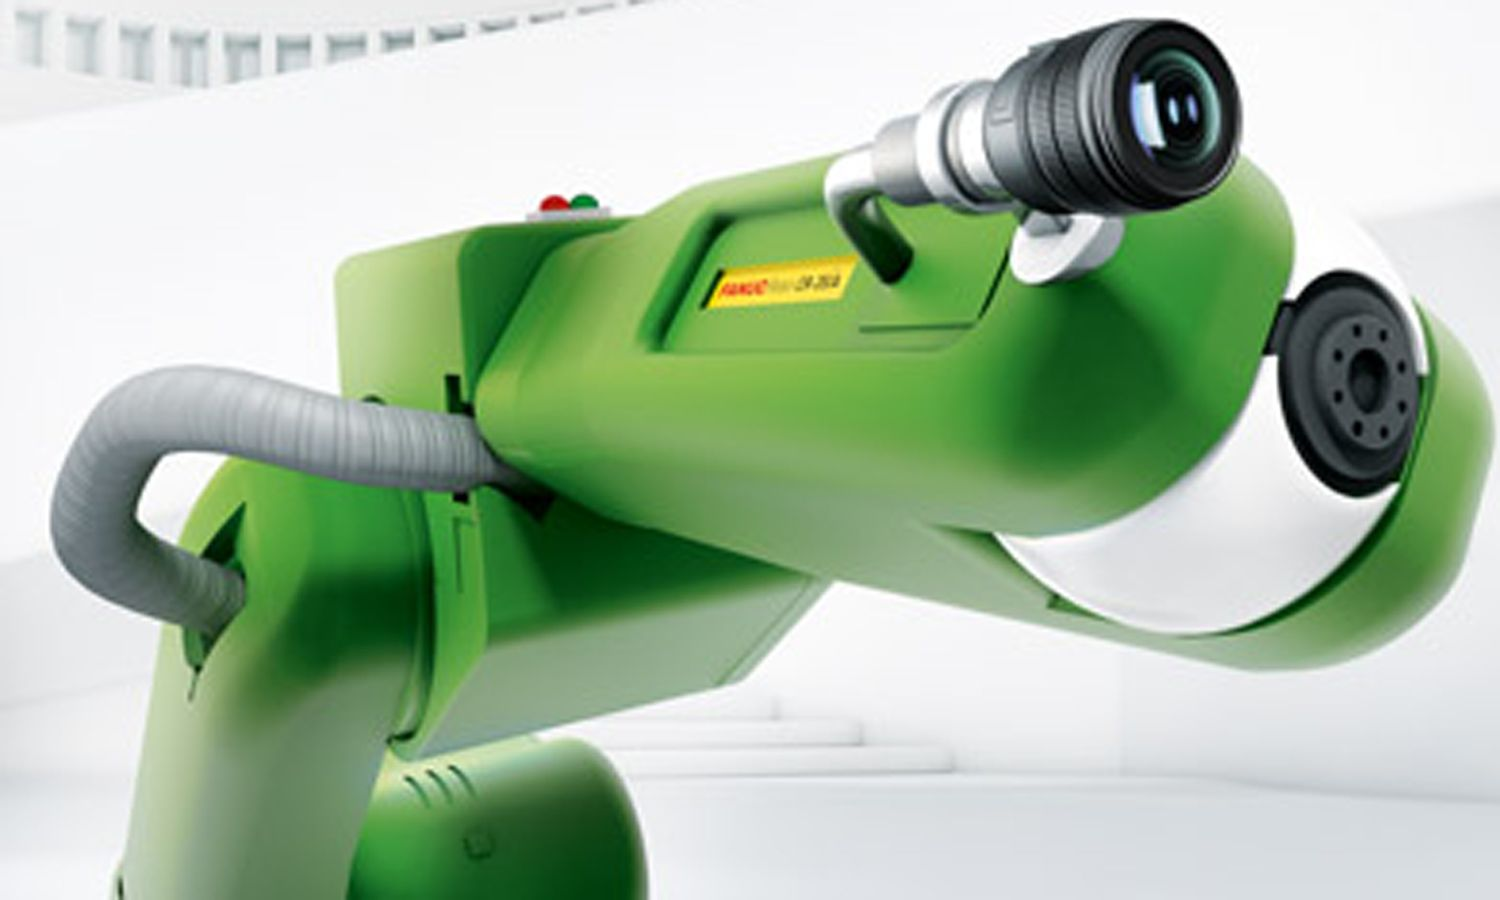
\includegraphics[scale=0.26]{images/fanuc_close.jpg}			% define cover picture
	\captionsetup{textformat=empty,labelformat=blank}
	\caption{Frontpage Picture \cite{fig:frontpage}}
	\end{figure}
\end{textblock}

\begin{textblock}{154}(28,133)
	\begin{picture}(150,2)
		\put(0,0){\color{bfhgrey}\rule{150mm}{2mm}}
	\end{picture}
\end{textblock}
\color{black}

% Institution / titel / subtitel / authors / experts:
%---------------------------------------------------------------------------
\begin{flushleft}

\vspace*{115mm}

\fontsize{26pt}{28pt}\selectfont 
\heading				\\							% Read heading from file leader/title.tex
\vspace{2mm}

\fontsize{16pt}{20pt}\selectfont\vspace{0.3em}
Preliminary Studies of Bachelor Thesis Rob195		\\				% Insert subheading
\vspace{5mm}

%\fontsize{10pt}{12pt}\selectfont
%\textbf{Description of thesis (semester- / Bachelor thesis / etc.)} \\		% Insert text
%\vspace{3mm}

% Abstract (eingeben):
%---------------------------------------------------------------------------
%\begin{textblock}{150}(28,190)
%\fontsize{10pt}{12pt}\selectfont
%[Insert short text (abstract) if desired] \\ 
%This document serves as a template for the compilation of reports according to the guidelines of the BFH. The template is written in LATEX and supports the automatic writing of various directories, references, indexing and glossaries. This small text is a summary of this document with a length of 4 to max. 8 lines. \\ 
%The cover picture may be turned on or off in the lines 157/158 of the file template.tex.
%\end{textblock}

\begin{textblock}{150}(28,225)
\fontsize{10pt}{17pt}\selectfont
\begin{tabbing}
	xxxxxxxxxxxxxxx\=xxxxxxxxxxxxxxxxxxxxxxxxxxxxxxxxxxxxxxxxxxxxxxx \kill
	Degree course:	\> Micro and Medical Technologies	\\		% insert name of degree course
	Author:		\> Aeschlimann Dario		\\					% insert names
	Tutors:	\> Rochat Sarah, Gruener Gabriel		\\							% insert names
	Constituent:	\> AHB Biel					\\							% insert names
	Experts:		\> Aigner Nikita				\\							% insert names
	Date:			\> \versiondate					\\							% read from file leader/version.tex
\end{tabbing}

\end{textblock}
\end{flushleft}

\begin{textblock}{150}(28,280)
\noindent 
\color{bfhgrey}\fontsize{9pt}{10pt}\selectfont
Berner Fachhochschule | Haute \'ecole sp\'ecialis\'ee bernoise | Bern University of Applied Sciences
\color{black}\selectfont
\end{textblock}


\end{titlepage}

%
% ===========================================================================
% EOF
%
		% activate for frontpage with picture
\cleardoubleemptypage
\setcounter{page}{1}
%\cleardoublepage
\phantomsection 

\chapter*{Management Summary}
\label{chap:managementSummary}

Lorem ipsum dolor sit amet, consectetur adipiscing elit. Phasellus scelerisque, leo sed iaculis ornare, mi leo semper urna, ac elementum libero est at risus. Donec eget aliquam urna. Lorem ipsum dolor sit amet, consectetur adipiscing elit. Nunc fermentum nunc sollicitudin leo porttitor volutpat. Duis ac enim lectus, quis malesuada lectus. Aenean vestibulum suscipit justo, in suscipit augue venenatis a. Donec interdum nibh ligula. Aliquam vitae dui a odio cursus interdum quis vitae mi. Phasellus ornare tortor fringilla velit accumsan quis tincidunt magna eleifend. Praesent nisl nibh, cursus in mattis ac, ultrices ac nulla. Nulla ante urna, aliquet eu tempus ut, feugiat id nisl. Nunc sit amet mauris vitae turpis scelerisque mattis et sed metus. Aliquam interdum congue odio, sed semper elit ullamcorper vitae. Morbi orci elit, feugiat vel hendrerit nec, sollicitudin non massa. Quisque lacus metus, vulputate id ullamcorper id, consequat eget orci \nocite{kopka:band1} \nocite{Marti06}. 

\cleardoubleemptypage
%---------------------------------------------------------------------------

% Table of contents
%---------------------------------------------------------------------------
\tableofcontents
\cleardoublepage
%---------------------------------------------------------------------------

% Main part:
%---------------------------------------------------------------------------
\pagenumbering{arabic}
\setstretch{1.25}
\chapter{Introduction}
\label{chap:introduction}
\setstretch{1.5}
Collaborative robots are meant to be flexible and easy to be reprogrammed so that they can be used efficiently in the modern industrial environment. One of the most important aspects for collaborative robots is safety. The robot shall not cause any harm to people or material. 
Currently there are three different types \cite{robotiq}  how the workspace of robots is monitored and protected from collisions:

\begin{itemize}
	\item Safety monitored stop: Scanners detect humans and objects inside the workspace of the robot and force a stop of any robot motion. This means the robot is not collaborative.
	\item Speed and separation monitoring: Scanners detect humans and objects inside certain areas around the robot and adjust the speed of the robot when the human comes closer to the robot. This leads to a stop of any robot motion when the human is coming too close to the robot. This is also referred to as cooperative operation.
	\item Power and force limiting: The robot is equipped with force and torque sensor to detect any abnormal forces applied to the robot body. Detecting such a force leads to a stop any robot motion. This type is called collaborative robot.Collisions can also be detected via a  sensitive skin on the robot. The skins can be pressure sensisitive or capacitive. The latter can detect flesh (they typically can not differentiate between a living human and a sausage) within a cm or two next to the skin. 
\end{itemize}
	
%	https://blog.robotiq.com/what-does-collaborative-robot-mean
Robots that rely on force sensors to detect collisions only recognize them and thus stopping any motion when the collision is already taking place. In a collaborative situation, the robot acts within a dynamic workspace and containers with liquids or heavy unstable objects may obstruct the workspace. These objects may be tipped over by the robot without triggering a halt or the halt could be triggered too late based on the force sensors, which could pose a health risk.
In addition, halts caused by the force sensors cause downtime in the production process which leads to higher production costs and longer production times, which companies like to avoid.
The goal of this thesis is to develop a vision system, which detects in real-time any occupied area in the workspace, that means people or objects which are within reach of the robot, and adapts the robots trajectories to avoid any collisions, thus providing an extra layer of safety. This would allow the robot to work in a modifiable workspace together with a human and to adapt his movements according to the human ones \cite{work_desc}. 

GPU-Voxels \cite{GPU-Voxels} is a similar project, that already has a vision system implemented to monitor the surroundings of various robots. It is mostly used in mobile robotics but has some implementations with an collaborative robots.

Commercially available camera based systems like the Pilz SafetyEye \cite{pilz} can recognize changes in the robot environment, however they do not have any capabilities to modify the robot's path.


\chapter{Tools}
\label{chap:tools}
\setstretch{1.5}
In this chapter an overview of the used robot, sensors, tools and software is given. Each section contains a brief description and hardware components include a specification list. Data sheets will be attached in the appendix.
\section{Hardware and Software}
\label{sec: hwsw}
\subsection{Fanuc CR-35iA}
\label{subsec:fanuc}
The Fanuc CR-35iA \cite{Fanuc} is one of the strongest collaborative robots currently available on the market. It can lift up to 35kg and has a maximum reach of 1.8m. The robot is designed to collaborate with humans on heavy and repetitive jobs in industries like automotive, packaging, distribution and metalworking. The robot body is coated with a soft rubber skin to prevent injuries and is ISO 10218-1:2011 certified. The certification specifies requirements and guidelines for the inherent safe design, protective measures and information for use of industrial robots. The robot is equipped with a Fanuc R-30iB controller. Figure \ref{fig:fanuc_human} shows the Fanuc CR-35iA besides the author for a size comparison.


\begin{figure}[H]
	\centering\includegraphics[scale=0.2]{images/robo_human.jpeg}			
	\caption{Fanuc CR-35iA robot side-by-side with a human for size comparison.}
	\label{fig:fanuc_human}
\end{figure}

%https://www.fanuc.eu/ch/en/robots/robot-filter-page/collaborative-robots/collaborative-cr35ia
%https://www.iso.org/standard/51330.html


\subsection{Asus Xtion PRO LIVE}
\label{subsec:asus}
The Asus Xtion PRO LIVE \cite{Asus} (figure \ref{fig:asus}) camera uses infrared sensors, adaptive depth detection technology and color image sensing to capture the user's real time image and movements. It is designed for gesture and whole body detection and has a set of predefined functions to support these tasks. The camera uses USB 2.0 Interface. The distance of use is between 0.8m and 3.5m. This camera was used since it was already available multiple times in the same version, the specifications meet the requirements and it was already used in similar projects.

\begin{figure}[H]
	\centering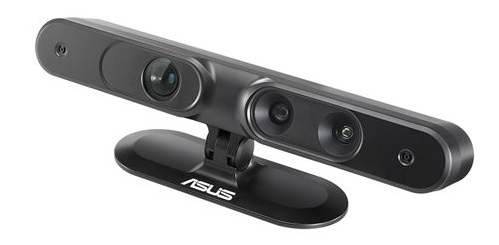
\includegraphics[scale=0.5]{images/Asus_Xtion_PRO_Live.jpg}			
	\caption{Asus Xtion PRO LIVE camera}
	\label{fig:asus}
\end{figure}


%http://xtionprolive.com/asus-3d-depth-camera/asus-xtion-pro-live

\subsection{Roboguide}
\label{subsec:roboguide}
Roboguide is an offline programming software for Fanuc robots. It allows the user to create programs for the robot and simulate its workspace in 3D without the physical need and expense of a prototype workspace setup. Two different types of programs can be used with the robot. Teach pendant or TP programs are mostly used for robot motions and calling other programs. TP programs can either be written on the teach pendant or within the Roboguide software. KAREL programs are used when the TP programs reach their limits. KAREL is a language very similar to Pascal. It features strongly typed variables, constants, custom types, functions and provides all sorts of built-ins for things which can't be done with TP. Karel is a compiled language, therefor the source must be translated from a KAREL file (.kl) into p-code (.pc) which is typically done in Roboguide. Roboguide and the two programming languages were used to establish a socket communication with an external C++ program. Figure \ref{fig:roboguide} shows the simulated workspace in Roboguide.

\begin{figure}[H]
	\centering\includegraphics[scale=0.3]{images/roboguide.png}			
	\caption{Simulated workspace environment in Fanuc Roboguide.}
	\label{fig:roboguide}
\end{figure}

\subsection{CloudCompare}
\label{subsec:cloudcomp}
CloudCompare is a 3D point cloud processing open source software. It has been originally designed to perform comparison between two dense 3D point clouds or between a point cloud and a triangular mesh. It relies on a specific octree data structure dedicated to this task. CloudCompare has been extended to a more generic point cloud processing software, including many advanced algorithms like registration, resampling and interactive or automatic segmentation. In this project, CloudCompare is used for the camera calibration process.

\begin{figure}[H]
	\centering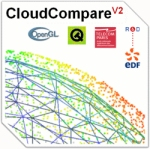
\includegraphics[scale=1]{images/cc_logo_v2_small.jpg}		
	\caption{CloudCompare logo.}
\end{figure}


\section{Libraries and Algorithms}
\label{sec:libalg}


\subsection{Point Cloud Library}
\label{subsec:pcl}
The Point Cloud Library (PCL) is a stand-alone, large scale, open project for 2D/3D image and point cloud processing. It is released under the  3-clause BSD license and thus free for commercial and research use. The PCL framework contains numerous state-of the art algorithms including filtering, surface reconstruction, registration, model fitting and segmentation. In this project, PCL is used to process the sensor data into point clouds, including filtering and transforming.

\begin{figure}[H]
	\centering
\includegraphics[scale=0.7]{images/pcl.png}			
	\caption{Point Cloud Library Logo.}
\end{figure}


\subsection{Octomap library}
\label{subsec:octomap} 
The Octomap library implements a 3D occupancy grid mapping approach, providing data structures and mapping algorithms in C++ particularly suited for robotics.  The map implementation is based on the octree data structure and is designed to provide a full 3D model with information about occupied, free and unknown cells. Information or new sensor readings can be added at any time and the extent of the map does not have to be known in advance. It is released under the  3-clause BSD license and thus free for commercial and research use.


\chapter{Methods}
\label{chap:method}                                   
\setstretch{1.5}                                       
\section{Robot Task}                                   
\label{sec: usecase}                                   
A pick and place application was created to test the collision avoidance system. The pick and place task is an endless loop, where the robot uses its vacuum gripper to move two wooden shingles from one side of the table to the other side and then back again. Figure \ref{fig:robotask} illustrates the robot movements with arrows pointing in the direction of the robot goal position.
                                                       
\begin{figure}[H]                                      
	\centering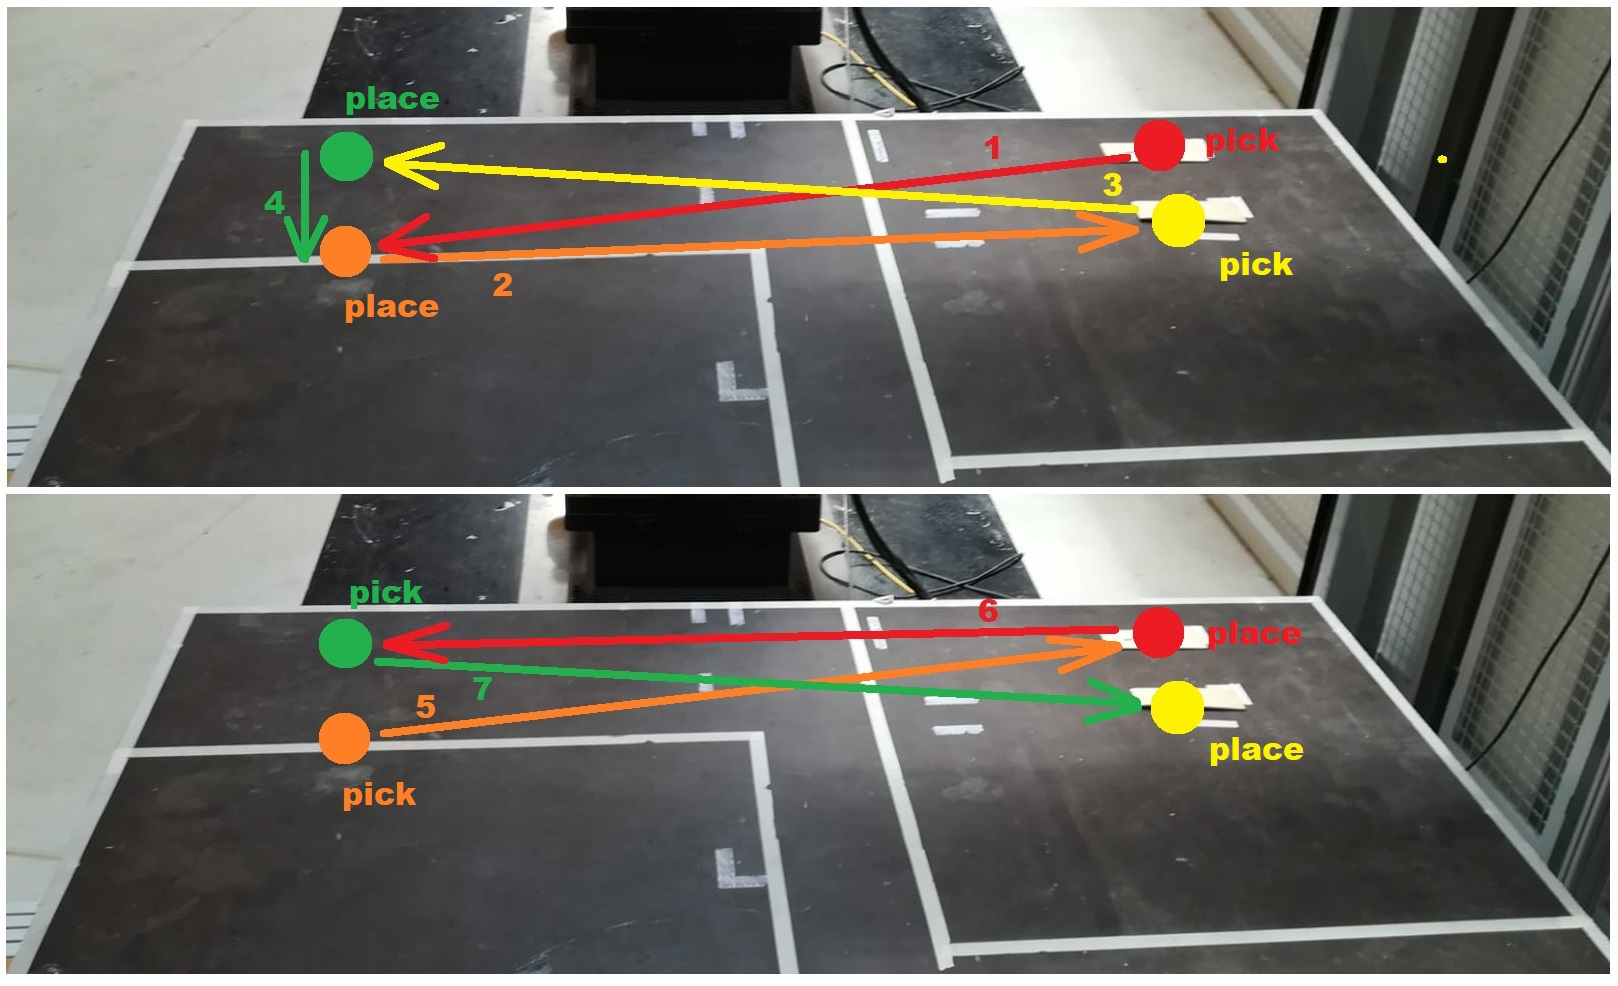
\includegraphics[scale=0.38]{images/robot_task.jpeg}		
	\caption{Robot task visualised.}   
	\label{fig:robotask}                    
\end{figure}                                           
\section{Robot communication}                          
\label{sec:robcom}                                     
As a first task, the communication between the collision avoidance system and the robot has to be established. A sequential communication approach was chosen since it provides a stable functionality and additional control over the process. The communication on the system side is run by a single TP program calling two KAREL programs, one for reading current robot positions of the robot, and one for writing go-to positions where the robot has to move to and and additional TP program to actually move the robot. The communication on the system side is provided by two functions written in C++. The sequential communication is run on the robot and uses flags in each of the KAREL and TP programs to trigger a certain function call. Listing \ref{lst:robcom} shows the TP program which runs the sequential communication TP program. The user frame and the tool are defined at program start. The position register is initialized with the correct type and the flags are set in their default value. The default value is set to be ready to send the current robot position to the collision avoidance system.
\begin{figure}[H]
\begin{lstlisting}[frame = single, caption={TP Program which enables the sequential communication.}, captionpos=b, label={lst:robcom}]
1:  UFRAME_NUM=8 ;
2:  UTOOL_NUM=3 ;
3:  PR[90]=LPOS    ;
4:  R[200]=(1) ;
5:  R[199]=(0) ;
6:  LBL[100] ;
7:  IF (R[200]=1 AND R[199]=0) THEN ;
8:  	CALL TEST_READ_C    ;
9:  ENDIF ;
10: IF (R[200]=0 AND R[199]=1) THEN ;
11:  	CALL TEST_WRITE_C    ;
12: ENDIF ;
13: IF (R[200]=0 AND R[199]=0) THEN ;
14:  	CALL ROS_MOVESM    ;
15: ENDIF ;
16: JMP LBL[100] ;
\end{lstlisting}
\end{figure} 				                                              
\subsection{Send and Read Robot Positions}   
          
\label{subsec:sendread}                                
\lstset{language=Pascal,
	basicstyle=\ttfamily,
	numbers=left,
	stepnumber=1,
	keywordstyle=\color{blue},
	stringstyle=\color{red},
	commentstyle=\color{green},
	morecomment=[l][\color{magenta}]{\#}
}          
The KAREL programs start with a header specifying different items like program name and environment settings. The KAREL programs of this project start both with almost exactly the same header part, only differentiating in the program name. Listing \ref{lst:karelhead} shows the file header of the read program.
\begin{figure}[H]
\begin{lstlisting}[frame = single, caption={KAREL header of the "read robot positions" function}, captionpos=b, label={lst:karelhead}]  
PROGRAM test_read_c
%STACKSIZE = 4000
%NOLOCKGROUP
%NOPAUSE=ERROR+COMMAND+TPENABLE
%ENVIRONMENT uif
%ENVIRONMENT sysdef
%ENVIRONMENT memo
%ENVIRONMENT kclop
%ENVIRONMENT bynam
%ENVIRONMENT fdev
%ENVIRONMENT flbt
%ENVIRONMENT REGOPE
%INCLUDE klevccdf
%INCLUDE klevkeys
%INCLUDE klevkmsk
\end{lstlisting}
\end{figure} 
\begin{tabbing}
	xxxxxxxxxxxxxxxxxxxxxxxxxxxx\=xxxxxxxxxxxxxxxxxxxxxxxxxxxxxxxxxxxxxxxxxxxxxxxxxxxxxxxxxxxxxxxxxx \kill
	PROGRAM:	\> Specifies the program name, max. 12 characters.	\\	
	\%STACKSIZE = n:		\>  Specifies the stack size in long words. \\				
	\%NOPAUSE = option:	\> Specifies a set of conditions which will  be prevented from pausing\\
						\>  the program. 		\\							% insert names
	\%ENVIRONMENT filename:	\> Used by the off-line translator to specify that a particular environment\\
					\> file should be loaded. 				\\	
	\%INCLUDE filename:		\>  Specifies files to insert into a program at translation time. 				\\							% insert names
	
\end{tabbing}
Listin \ref{lst:karelseq1} shows the second part of the KAREL program which specifies variables, which will be used during program execution.
\begin{figure}[H]
\begin{lstlisting}[frame = single, caption={KAREL variable definitions}, captionpos=b, label={lst:karelseq1}]
VAR
file_var   : FILE
STATUS  : INTEGER
entry   : INTEGER
cur_pos: XYZWPR		-- Robot position
-- REAL Array to convert to robot position
c_real_array : ARRAY[6] OF REAL  
indx   : INTEGER    --for counter

CONST
-- POS Register Number wich will be used to store the current
   robot position
MOVE_PREG = 90
-- Flags to indicate which step is next. used in ROB195_COM.ls
WRITE_FLAG = 199
READ_FLAG = 200
\end{lstlisting}
\end{figure} 
After the variable definitions the actual program sequence starts by setting up the server port and opening the file variable to write the current robot position as shown in listing \ref{lst:karelconnect}. The port 59004 is used for the read command and port 59003 is used for the write command.
\begin{figure}[H]
\begin{lstlisting}[frame = single, caption={KAREL start connection to client.}, captionpos=b, label={lst:karelconnect}]
BEGIN
indx = 1	
FORCE_SPMENU(TP_PANEL,SPI_TPUSER,1)
WRITE TPDISPLAY (CHR(128),CHR(137))
SET_FILE_ATR(file_var, ATR_IA)
-- set the server port before doing a connect
SET_VAR(entry, '*SYSTEM*',
  '$HOSTS_CFG[3].$SERVER_PORT',59004,STATUS)
WRITE TPDISPLAY('Connecting..',CR)
MSG_CONNECT('S3:',STATUS) -- connecting to system
WRITE TPDISPLAY(' CONNECT STATUS = ',STATUS,CR)
IF STATUS = 0 THEN -- checks connection status
-- Open S3:
	WRITE TPDISPLAY('Opening',CR)
	OPEN FILE file_var ('rw','S3:')
	STATUS = IO_STATUS(file_var)
	WRITE TPDISPLAY(STATUS,CR)
\end{lstlisting}
\end{figure}

When the connection is successful, the current robot position is written to the cur\_pos variable using the CURPOS built-in function, which returns the XYZ coordinates as well as the WPR angles. The current position needs then to be written into the real array in order to write it to the file variable and send it to the system. 
\begin{figure}[H]
\begin{lstlisting}[frame = single, caption={KAREL read current robot position and prepare the data for sending.}, captionpos=b, label={lst:karelvarprep}]
 IF STATUS = 0 THEN
-- write an integer
	cur_pos = CURPOS(0,0)
	
	c_real_array[1] = cur_pos.X
	c_real_array[2] = cur_pos.Y
	c_real_array[3] = cur_pos.Z
	c_real_array[4] = cur_pos.W
	c_real_array[5] = cur_pos.P
	c_real_array[6] = cur_pos.R
\end{lstlisting}
\end{figure}
After preparing the position data, it is sent using a for statement to loop through the REAL array and send each coordinate. Afterwards the file variable is closed and the client is disconnected. The flags are set in order to start the writing step.
\begin{figure}[H]
\begin{lstlisting}[frame = single, caption={KAREL sending position data and closing connection.}, captionpos=b, label={lst:karelread}]
		FOR indx = 1 TO 6 DO
			WRITE file_var(c_real_array[indx], CR)
		ENDFOR
		CLOSE FILE file_var
	ENDIF
	WRITE TPDISPLAY('Disconnecting..',CR)
	MSG_DISCO('S3:',STATUS)
	WRITE TPDISPLAY('Done.',CR)
	SET_INT_REG(WRITE_FLAG, 1, STATUS)
	SET_INT_REG(READ_FLAG, 0, STATUS)
ENDIF
END test_read_c
\end{lstlisting}
\end{figure}
The write command is build in the same manner but reverses the steps. This means the position is written into the real array and then converted to the position variable, which is then stored in the position register of the robot controller. The code can be found in the appendix \ref{app:karelread} on page \pageref{app:karelread}. The program for the read and write functions is based on the socket communication example from the KAREL reference manual for the R-30iA controller \cite{refman}.

The systems uses two C++ functions to either read position data from the robot or write goal positions for the robot. Listing \ref{lst:cppread1} shows the first part of the read function, where the host address and port are set up.

\lstset{language=C++,
	numbers=left,
	stepnumber=1,
	basicstyle=\ttfamily,
	keywordstyle=\color{blue},
	stringstyle=\color{red},
	commentstyle=\color{green},
	morecomment=[l][\color{magenta}]{\#}
}
\begin{figure}[H]
\begin{lstlisting}[frame = single, caption={C++ Set up host adress and port.}, captionpos=b, label={lst:cppread1}]
float *connectReadCartesian (float *current_cartesian_pos){
// READ SETUP
	int sockfd;
	struct sockaddr_in serv_addr_read;
	bzero((char *) &serv_addr_read, sizeof(serv_addr_read));
	serv_addr_read.sin_family = AF_INET;
	serv_addr_read.sin_addr.s_addr = inet_addr(SERV_HOST_ADDR);
	serv_addr_read.sin_port = htons(SERV_TCP_PORT_READ);
\end{lstlisting}
\end{figure}
Listing \ref{lst:cppread2} shows the second part of the read function, where the client connects to the host. When the connection is successful, the \emph{readPos()} function is called, which reads the six parts of the robot position, each character separately.
\begin{figure}[H]
\begin{lstlisting}[frame = single, caption={C++ connect to host and read current robot position.}, captionpos=b, label={lst:cppread2}]
// READ POS

	if((sockfd = socket(AF_INET, SOCK_STREAM,0)) < 0){
	  printf("Client: Can't Open Stream Socket\n");
	}
	printf("Client: Connecting to READ server...\n");
	  while(connect(sockfd,(struct sockaddr *) ...
		   &serv_addr_read, sizeof(serv_addr_read))<0){
	  printf("Client: Can't Connect to the READ server\r");
	}

	printf("Client: Connected!\n");
	current_cartesian_pos = readPos(sockfd);

	return current_cartesian_pos;
}
\end{lstlisting}
\end{figure}
Writing goal positions for the robot has the same functionality as reading the positions, but again in reverse. Each character of the six coordinates separately. The code for the write function can be found in appendix \ref{app:com_func.cpp}.
                       
\subsection{Robot movements}
\label{subsec:robmove}

\lstset{language=Pascal,
	basicstyle=\ttfamily,
	numbers=left,
	stepnumber=1,
	keywordstyle=\color{blue},
	stringstyle=\color{red},
	commentstyle=\color{green},
	morecomment=[l][\color{magenta}]{\#}
}       
The robot movements are done by using the linear movement function provided by the built-in library of Fanucs TP programming language. Listing \ref{lst:robmove} shows the TP program, which moves the robot to the specified position in the position register \#90. First it defines the tool and the frame in which the robot should move. Then the linear movement is specified by its end position, speed and if the point is a fixed point or a via point. FINE states that the point is a fixed point which has to be exactly reached. The flags R[200] and R[199] are used to trigger the next step of the sequence of the communication.
\begin{figure}[H]
\begin{lstlisting}[frame = single, caption={TP Move the robot the the specified position.}, captionpos=b, label={lst:robmove}]
1:  UTOOL_NUM=3 ;
2:  UFRAME_NUM=8 ;
3:L PR[90] 250mm/sec FINE ;
5:  R[200]=(1) ;
6:  R[199]=(0) ;
\end{lstlisting}
\end{figure}
\subsection{Gripping commands}
\label{subsec:gripcom}
\lstset{language=[5.3]LUA,
	numbers=left,
	stepnumber=1,
	basicstyle=\ttfamily,
	keywordstyle=\color{blue},
	stringstyle=\color{red},
	commentstyle=\color{green},
	morecomment=[l][\color{magenta}]{\#}
}
Usually the gripping commands would be executed using fieldbus communication. However, currently no working fieldbus communication is available on the robot. 

In order to have a very simple communication to send gripping commands, two simple LUA scripts (listing \ref{lst:telnet}) were written, each connecting to the robot controller over telnet writing a specified value to a digital out of the robot, that activates the gripper.
\begin{figure}[H]
\begin{lstlisting}[frame = single, caption={LUA Script for telnet connection.}, captionpos=b, label={lst:telnet}]  
  --set up telnet conn
local ip = '147.87.144.251';
local port = 23; -- TELNET
local sock = require('socket');
local serv, err = sock.connect(ip, port);
local action = 0 -- actual gripping command
--actuation
serv:send('LOGIN\r');
sock.sleep(0.15);
serv:send('PASSWORD\r');
sock.sleep(0.15);
serv:send('set port rdo[7]='.. action.. '\r');
sock.sleep(0.25);
serv:close();
\end{lstlisting}
\end{figure}
The two LUA scripts only differ in the value of the variable "local action" on listing \ref{lst:telnet} on line six. A "0" is used to disable the vacuum of the gripper, and a "1" is used to enable the gripper vacuum. In order to improve code readability, two C++ functions were implemented named gripperOn (listing \ref{lst:gripON})/ gripperOff (listing \ref{lst:gripOFF}) located in the com\_func.cpp file.

\lstset{language=C++,
	numbers=left,
	stepnumber=1,
	basicstyle=\ttfamily,
	keywordstyle=\color{blue},
	stringstyle=\color{red},
	commentstyle=\color{green},
	morecomment=[l][\color{magenta}]{\#}
}
\begin{figure}[H]
\begin{lstlisting}[frame = single, caption={gripperOn function}, captionpos=b, label={lst:gripON}]  
void gripperOn (void){
	system("lua5.3 ../Rob195/1.txt");
}
\end{lstlisting}
\end{figure}
\begin{figure}[H]
\begin{lstlisting}[frame = single, caption={gripperOff function}, captionpos=b, label={lst:gripOFF}]  
void gripperOff (void){
	system("lua5.3 ../Rob195/0.txt");
}
\end{lstlisting}
\end{figure}
\section{Data gathering, workspace monitoring}
\label{sec:datagather}
\subsection{Camera positioning}
\label{subsec:campos}
The original camera design did not allow to mount the camera with screws in a fixed position as seen in figure \ref{fig:asus} in section \ref{subsec:asus}. In order to be able to do so, a fixture piece was designed using the CAD Software NX \cite{NX}. The fixture allows the camera to be fixed in any desired angle. Since the fixture doesn't have any requirements regarding applied forces or stability except for holding the camera, the piece was 3D printed.

\begin{figure}[H]                                      
	\centering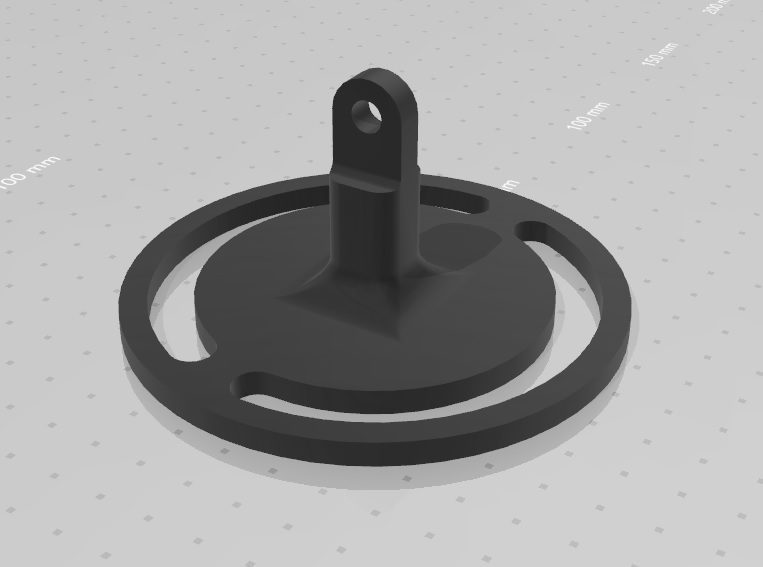
\includegraphics[scale=0.45]{images/halter.jpg}			
	\caption{camera fixture design.}
	\label{fig:camfix}                      
\end{figure}

To mount the cameras, item profiles \cite{Item} were used to build a simple structure to position the cameras.

It was not possible to monitor the whole workspace with only two cameras, so only one side of the robot workspace is monitored. The cameras were placed diagonally over the table which is placed inside the workspace as shown in Figure  \ref{fig:campos}.

\begin{figure}[H]                                      
	\centering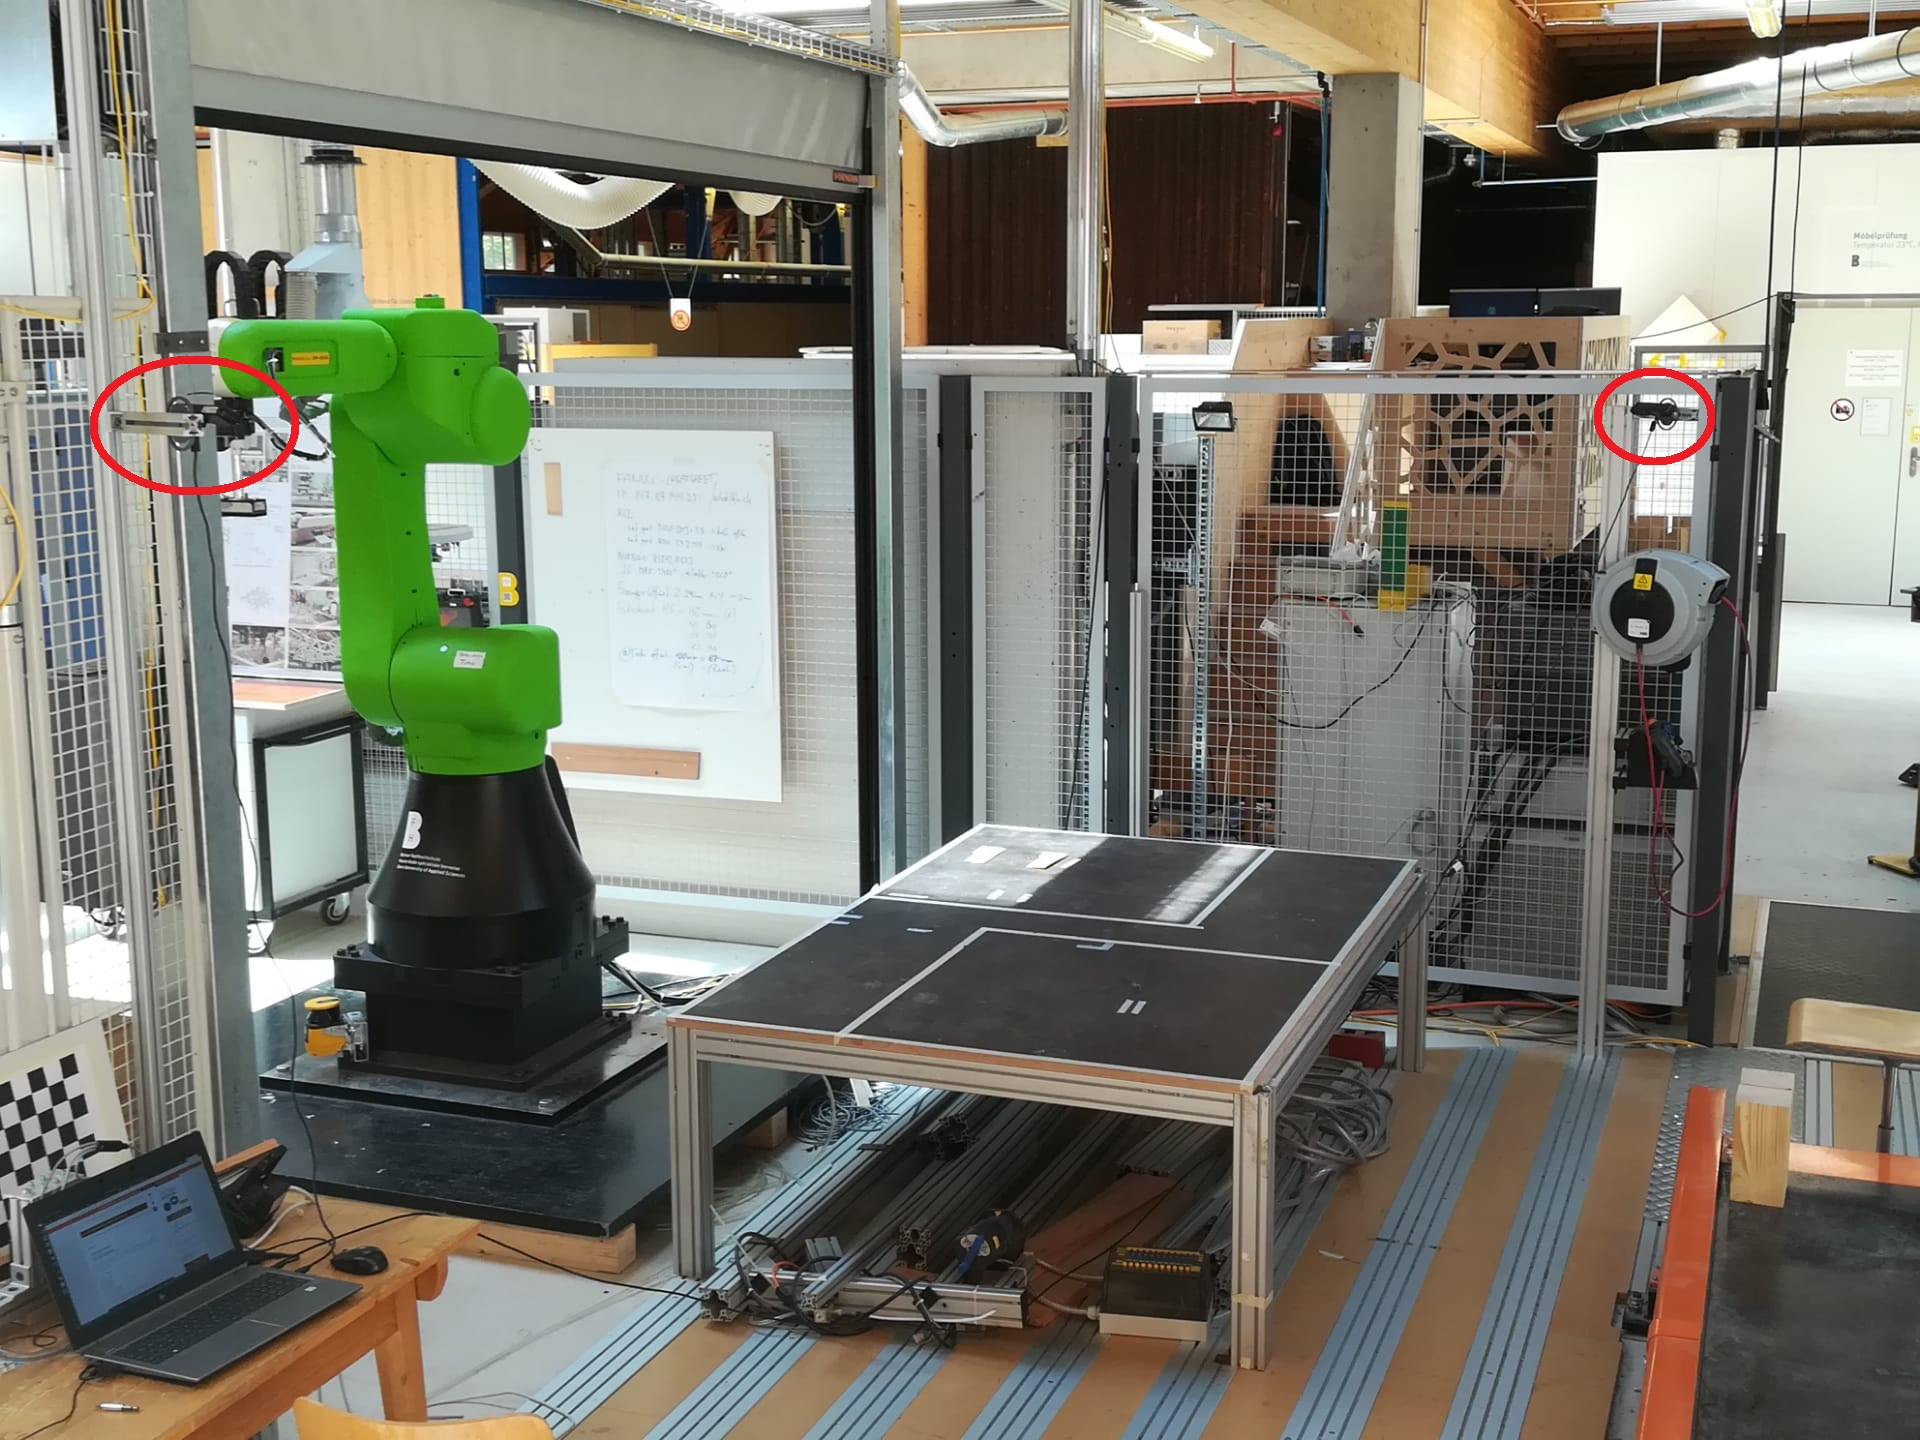
\includegraphics[scale=0.2]{images/campos.jpeg}			
	\caption{Final camera positions, cameras are marked red.}
	\label{fig:campos}                      
\end{figure}
 The diagonal positioning was chosen in order to have any side of objects on the table visible in the camera view. In a first approach the cameras were set up right beside the table, but since the projected infrared pattern of each camera interferes with each other, the cameras were moved further away from each other to reduce the intensity\cite{cameraInterference} of the infrared structure and thus to reduce the interference.

The interference of the cameras resulted in loss of data, but only on horizontal surfaces. The sides of the objects were still recognised, since each side of the object is only visible by a certain camera. Figure \ref{fig:infrared} shows the infrared pattern and how it behaves with obstacles in it.

%http://www.robotics.tu-berlin.de/fileadmin/fg170/Publikationen_pdf/martinmartin_14_ki_iros.pdf

\begin{figure}[H]                                      
	\centering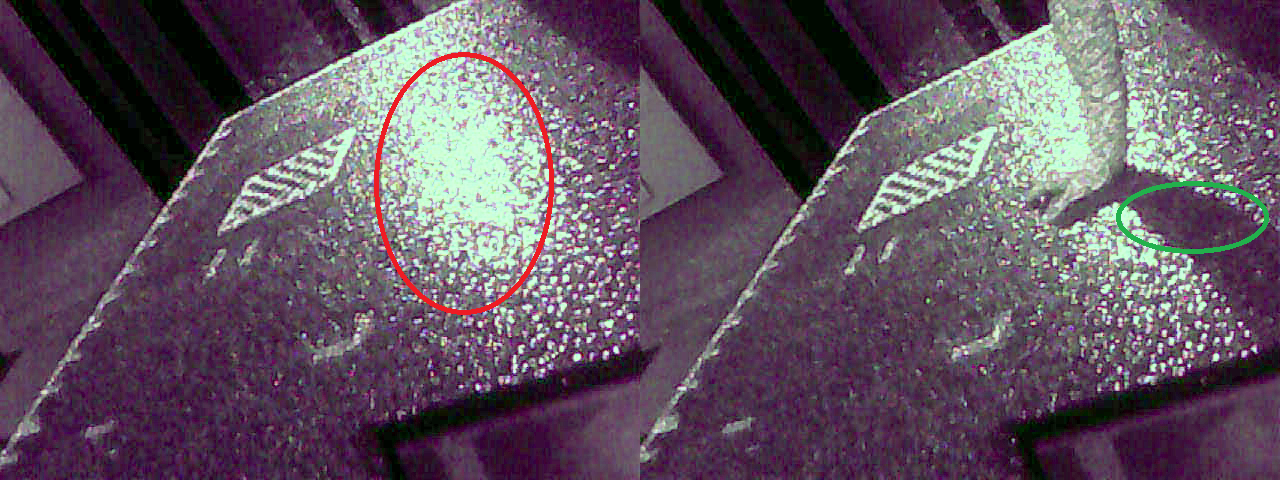
\includegraphics[scale=0.5]{images/Infrared.png}			
	\caption{Infrared structure capture. On the left side the interference, which results ins data loss, is marked in red. Green marked is the area which is inside the object shadow of one camera.}
	\label{fig:infrared}                      
\end{figure}

\subsection{Camera calibration}
\label{subsec:camcalib}
\lstset{language=C++,
	basicstyle=\ttfamily,
	keywordstyle=\color{blue},
	stringstyle=\color{red},
	commentstyle=\color{green},
	morecomment=[l][\color{magenta}]{\#}
}
The calibration of the cameras is done using CloudCompare and its possibility to align multiple point clouds to each other. For this a reference point cloud of the table (Figure \ref{fig:refpctable}) is generated when executing the camCalibration program. The program creates a point cloud with the surface of the table in red color. The two marked squares on the table are marked blue in the point cloud. For axis recognition a small green surface is created below the table (negative Z-direction). The table reference cloud is created at the position in the world frame of the robot.

\begin{figure}[H]                                      
	\centering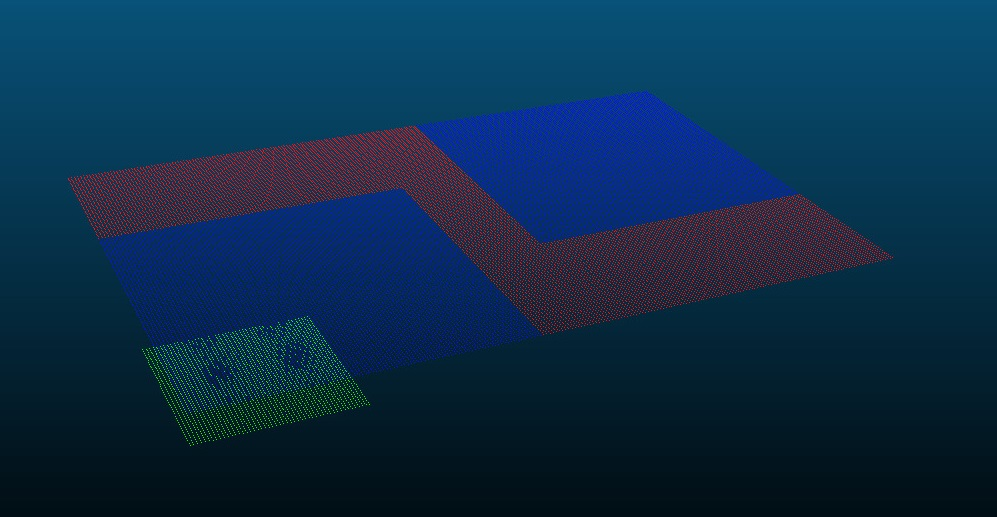
\includegraphics[scale=0.5]{images/CC_tableref.jpeg}			
	\caption{Reference point cloud of the table surface}
	\label{fig:refpctable}                      
\end{figure}

In addition a point cloud capture of the robot workspace from each camera is generated when the program is executed. The calibration is then done by loading the three point clouds into Cloud Compare and using the "Align two point clouds by picking (at least 4) equivalent points" command, which is located at in the top bar of Cloud Compare as marked with a red circle in figure \ref{fig:showpoints}. After clicking on the command button, a window appears in which the reference cloud can be set. Be sure to select the table reference cloud as reference.

\begin{figure}[H]                                      
	\centering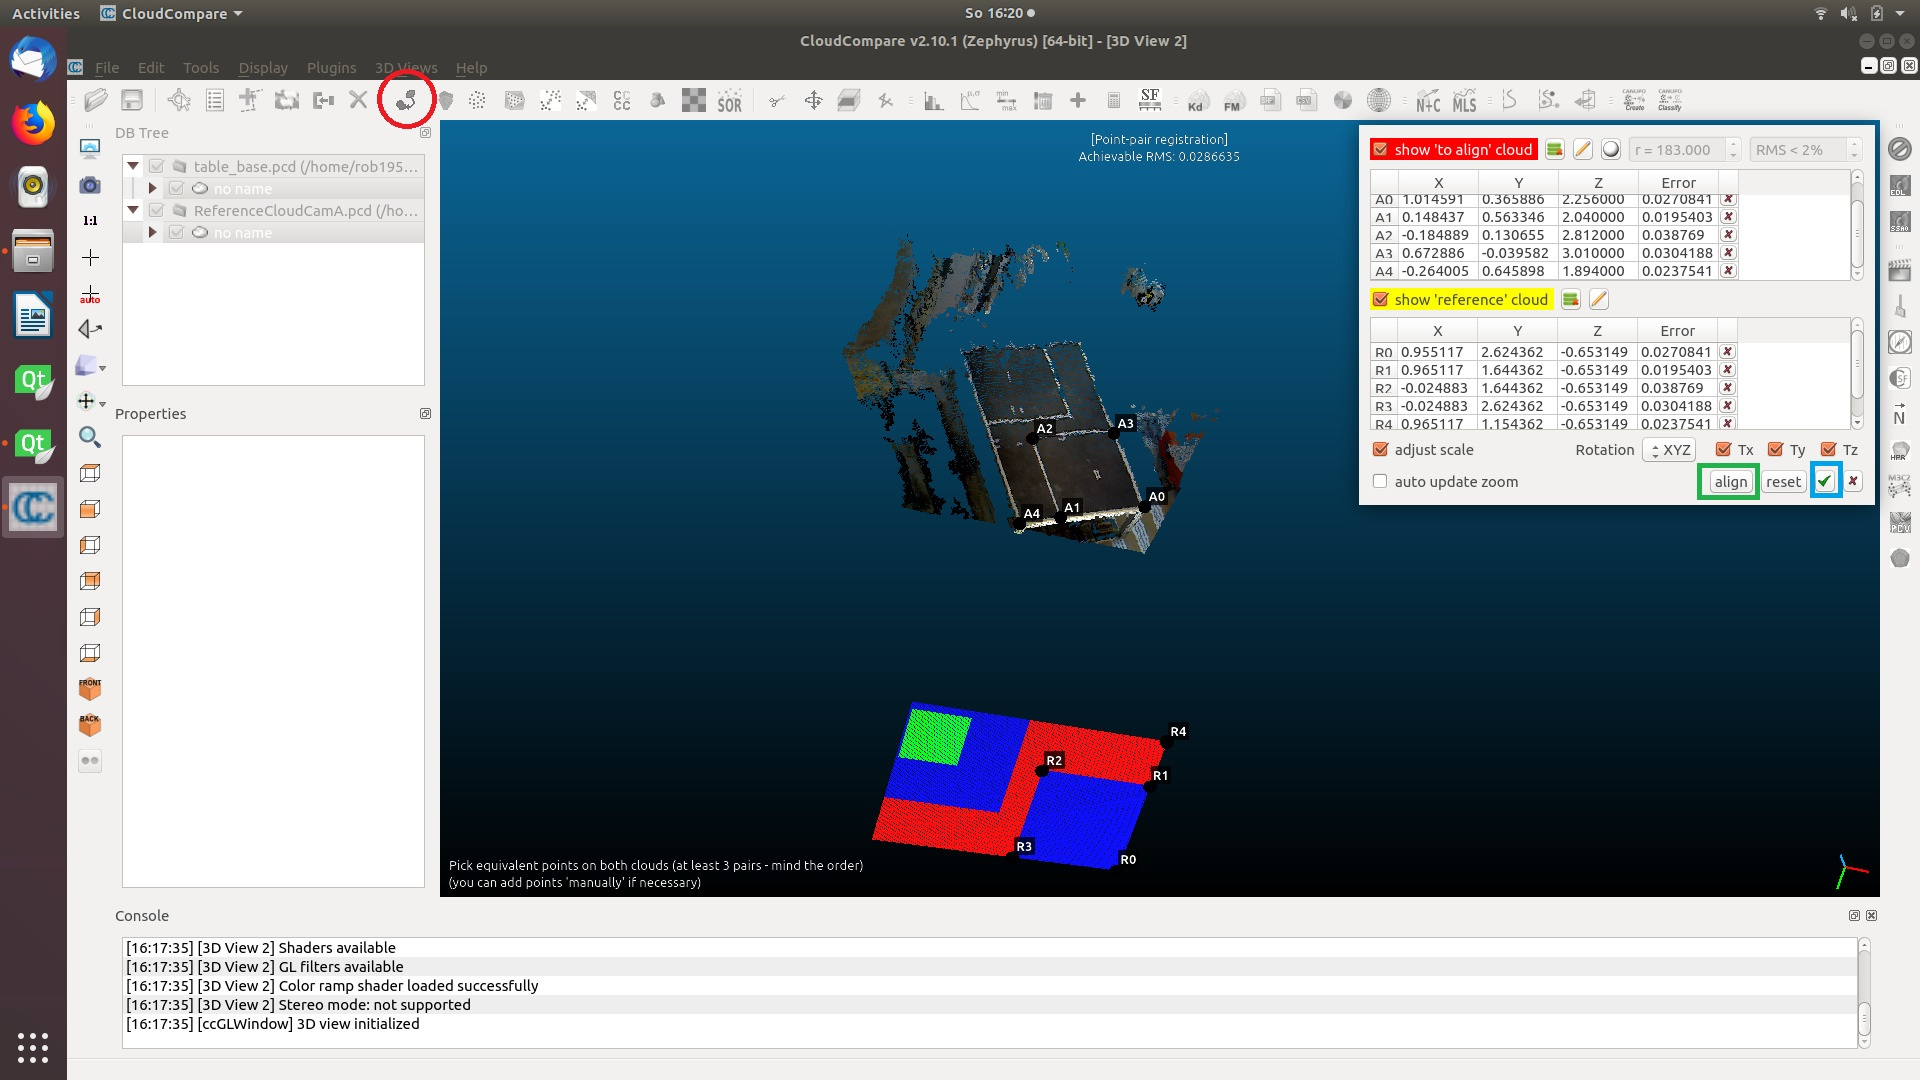
\includegraphics[scale=0.28]{images/CC_show_points.jpeg}			
	\caption{Table reference point cloud and a single camera generated poit cloud. Red Mark shows the "align" command. After picking the points the green marked "align" button can be clicked to show the result of the command. By clicking on the blue marked "approve" button, the changes are applied.}
	\label{fig:showpoints}                      
\end{figure}

\begin{figure}[H]                                      
	\centering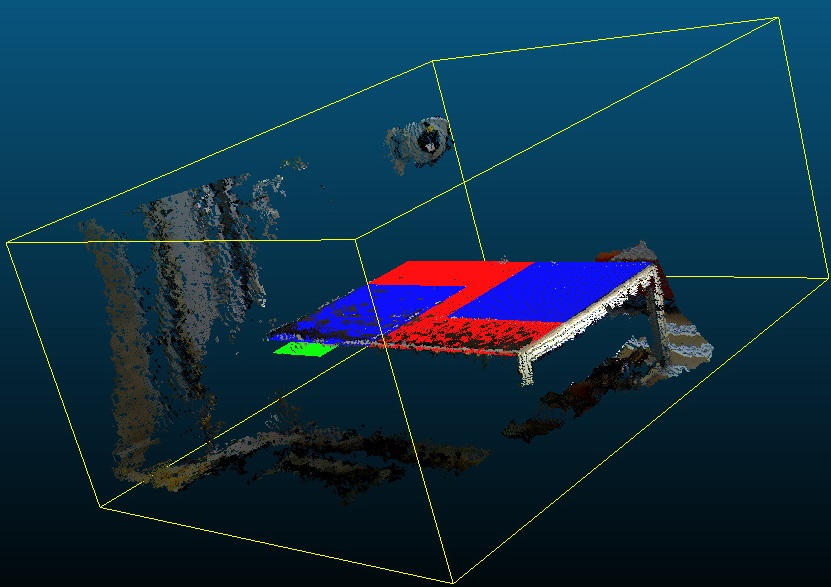
\includegraphics[scale=0.5]{images/CC_aligned_cloud.jpeg}			
	\caption{Single camera generated point cloud aligned with the table reference cloud.}
	\label{fig:cloudaligned}                      
\end{figure}

Figure \ref{fig:cloudaligned} shows a single point cloud aligned with the table reference. After aligning both camera generated point clouds, the transformation matrix can be found on the properties window, after selecting the specific point cloud, on the left side of Cloud Compare. This matrix can then be copied and pasted into the "cloudA.txt" respectively the "cloudB.txt" file, located in the Software/Rob195 folder. The matrices are then read into the collision avoidance software at the start of the main function (listing \ref{lst:matrixread}).
\begin{figure}[H]
\begin{lstlisting}[frame = single, caption={part of the main function of the collision avoidance system which reads the transformation matrices for camera A and B.}, captionpos=b, label={lst:matrixread}]  
// read cloud transformation data from file
ifstream fin ("./../Rob195/cloudA.txt");

if (fin.is_open()){
	for (int row = 0; row < nrows; row++){
		for (int col = 0; col < ncols; col++){
			float item = 0.0;
			fin >> item;
			transformCamA(row, col) = item;
		}
	}	
	fin.close();
}
ifstream fin2 ("./../Rob195/cloudB.txt");
if (fi2n.is_open()){
	for (int row = 0; row < nrows; row++){
		for (int col = 0; col < ncols; col++){
			float item = 0.0;
			fin2 >> item;
			transformCamB(row, col) = item;
		}
	}
	fin2.close();
}
\end{lstlisting}
\end{figure}
\subsection{Data acquisition}
\label{subsec:dataacq}

For the data acquisition the cameras were run using the OpenNI Grabber Framework in PCL. The simple openNI viewer class is available from the tutorials of the PCL. The example file was used and adapted to support a second camera. The \emph{run()} method of the class, creates for each camera a new OpenNIGrabber interface (listing \ref{lst:interface}). 
\lstset{language=C++,
	numbers=left,
	stepnumber=1,
	keywordstyle=\color{blue},
	stringstyle=\color{red},
	commentstyle=\color{green},
	morecomment=[l][\color{magenta}]{\#}
}
\begin{figure}[H]
\begin{lstlisting}[frame = single, caption={part of the run() function of the simple openNI viewer class}, captionpos=b, label={lst:interface}]  
 void run (){
	//**********************************
	//        start first Xtion
	Grabber* interface = new io::OpenNI2Grabber("#1");

	boost::function<void (const pcl::PointCloud
		<pcl::PointXYZRGBA>::ConstPtr&)> f =
	boost::bind (&SimpleOpenNIViewer::cloud_cb_, this, _1);

	interface->registerCallback (f);
	interface->start();
	//**********************************
	//**********************************
	//        start second Xtion
	pcl::Grabber* interface2 = new io::OpenNI2Grabber("#2");
	boost::function<void (const pcl::PointCloud
		<pcl::PointXYZRGBA>::ConstPtr&)> f2 =
	boost::bind (&SimpleOpenNIViewer::cloud_cb_2_, this, _1);

	interface2->registerCallback (f2);
	interface2->start();
	//**********************************
\end{lstlisting}
\end{figure}
\emph{pcl::PointCloud<pcl::PointXYZRGBA>::ConstPtr \&cloud} defines a pointer to a point cloud with color values (listing \ref{lst:callbackdef}). \emph{pcl::PointXYZ} would define a point cloud without color values. 
\begin{figure}[H]
\begin{lstlisting}[frame = single, caption={Function definition of the callback function, using a pointer to a point cloud with color values.}, captionpos=b, label={lst:callbackdef}]  
void cloud_cb_ (const pcl::PointCloud
	<pcl::PointXYZRGBA>::ConstPtr &cloud)
\end{lstlisting}
\end{figure}
The callback methods \emph{cloud\_cb\_()} and \emph{cloud\_cb\_2\_()} create at first a range filter to remove data which is out of bounds. This is realised with the \emph{pcl::PassThrough} object as shown in listing \ref{lst:passfilter}. The passthrough filter can be set up to specify in which axis the data needs to be filtered and at what range the data should be filtered. Be aware that for the set up of the filter the camera frame is used and the units used are meters. \emph{pass.setFilterLimitsNegative (true)} could be used to inverse the filter.
\begin{figure}[H]
\begin{lstlisting}[frame = single, caption={Passthrough filter for the camera input, to remove data which is out of bounds.}, captionpos=b, label={lst:passfilter}]  
pcl::PointCloud<pcl::PointXYZRGBA>::Ptr 
  CloudCamAfiltered (new pcl::PointCloud<pcl::PointXYZRGBA> ()); 
 // filter element
pcl::PassThrough<pcl::PointXYZRGBA> pass; 
pass.setInputCloud (cloud);
// axis definition
pass.setFilterFieldName ("z");	
// range definition, points from start to endpoint are included	
// in the pointcloud, the rest is filtered out.
pass.setFilterLimits (0.0, 4.1);

// pass.setFilterLimitsNegative (true);

// output cloud
pass.filter (*CloudCamAfiltered); 	
\end{lstlisting}
\end{figure}
After filtering out points out of bounds, the point clouds are downsampled using a voxelgrid filter element. This implements the octree data structure. The octree is a tree data structure in which each internal node has exactly eight children. The root node describes a cubic bounding box which encapsulates all points from the point cloud. By dividing this cube into eight smaller cubes, each representing a certain part of the root cube, the next level of the octree is generated as shown in figure \ref{fig:octree}. The node is always the center point of the cube it is representing. Processing a point cloud into an octree data structure already provides a form of voxelizing. The resolution can be chosen by defining how many layers the octree data structure should have or by defining the size of the cubes at the lowest level of the octree. 

\begin{figure}[H]                                      
	\centering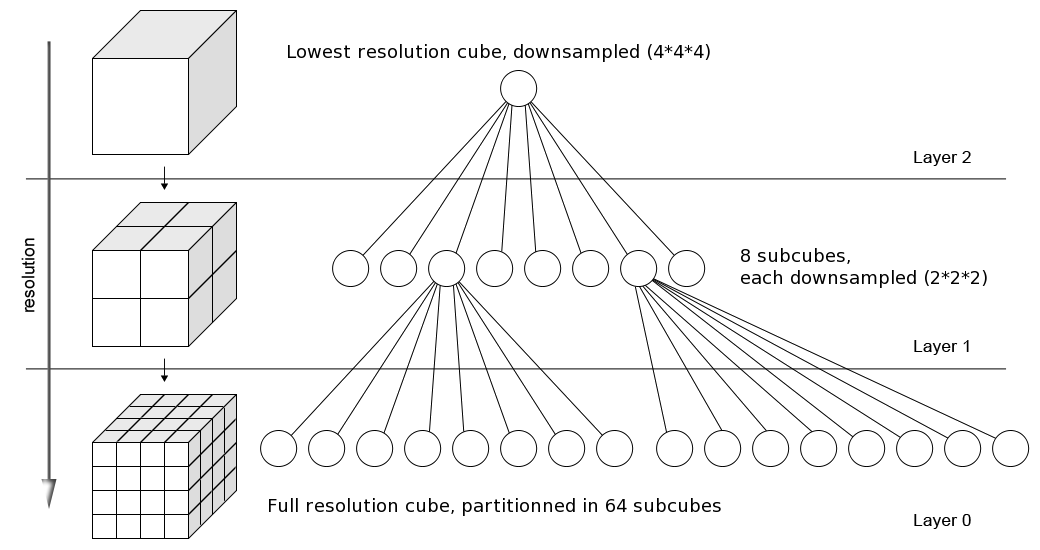
\includegraphics[scale=0.4]{images/Octree.png}			
	\caption{Graphical Illustration of an octree data structure}
	\label{fig:octree}                      
\end{figure}
\begin{figure}[H]
\begin{lstlisting}[frame = single, caption={Voxelgrid filter to downsample the point cloud and reduce the total amount of points.}, captionpos=b, label={lst:voxelfilter}]  
pcl::PointCloud<pcl::PointXYZRGBA>::Ptr 
   CloudCamAVoxelGrid (new pcl::PointCloud<pcl::PointXYZRGBA> ()); 
// filter element
pcl::VoxelGrid<pcl::PointXYZRGBA> voxelFilter; 
voxelFilter.setInputCloud(CloudCamAfiltered);
// cube size definition in meters
voxelFilter.setLeafSize (0.01f, 0.01f, 0.01f); 
// output cloud
voxelFilter.filter (*CloudCamAVoxelGrid); 
\end{lstlisting}
\end{figure}
After filtering, the point clouds are transformed to their exact position by using the previously generated transform matrices. This is done by using the \emph{pcl::transformPointCloud (*CloudCamAVoxelGrid, *transformedCloudCamA, transformCamA);} command. As parameters the input cloud, the output cloud and the transformation matrix have to be given to the function.

After transformation the point clouds are saved to the disk, when the program is executed with the debug flag (-d).

\section{Data processing and mapping}
\label{sec:process}
After the point clouds are pre-filtered and transformed into the necessary frame, a single point cloud is generated by concatenating (listing \ref{lst:concatenate}) the data from camera A and B. This is done inside the \emph{run()} function of the simpleOpenNIviewer class.
\begin{figure}[H]
\begin{lstlisting}[frame = single, caption={merging the point clouds from camera A and B into a single point cloud by concatenating the data.}, captionpos=b, label={lst:concatenate}]
*concatenatedCloud = *transformedCloudCamA;
*concatenatedCloud += *transformedCloudCamB;
\end{lstlisting} 
\end{figure}
The merged point cloud is then filtered again into the actual desired size of the cubes for the occupancy grid. The reason the merged point cloud is filtered again is simply due to avoid having data points close to each other by merging the point clouds from camera A and B. Since both cameras capture the same picture from a different angle, it is possible to have multiple points on the same spot. After applying the filter, an empty occupancy grid is created and afterwards filled with the data points from the merged point cloud. For this project a leaf size of 0.04m has been chosen since bigger leaf sizes appeared too big and inaccurate while lower leaf sizes resulted in longer calculating time. Figure \ref{fig:occupamcy} shows an occupancy grid created by the system.
\begin{figure}[H]
\begin{lstlisting}[frame = single, caption={Creating an empty occupancy grid of a specified leaf size. Then filling it with th point cloud data}, captionpos=b, label={lst:emptymap}]  
// creating map object and defining its leaf size
octomap::ColorOcTree tree( 0.04 ); 
for (float x = -2.5; x <= 2.5; x += 0.08f) { 
	for (float y = 0; y <= 4; y += 0.08f) {
		for (float z = -1.5; z <= 2; z += 0.08f) {
			octomap::point3d endpoint(x, y, z);
			// integrate 'free' measurement
			tree.updateNode(endpoint, false); 
		}
	}
}

//filling map with point cloud data
for (auto p:cloud_filtered->points){
	tree.updateNode(octomap::point3d(p.x, p.y, p.z), true);
}
// adding color information
for (auto p:cloud_filtered->points){
	tree.integrateNodeColor( p.x, p.y, p.z, p.r, p.g, p.b );
}
\end{lstlisting}
\end{figure}
\begin{figure}[H]                                      
	\centering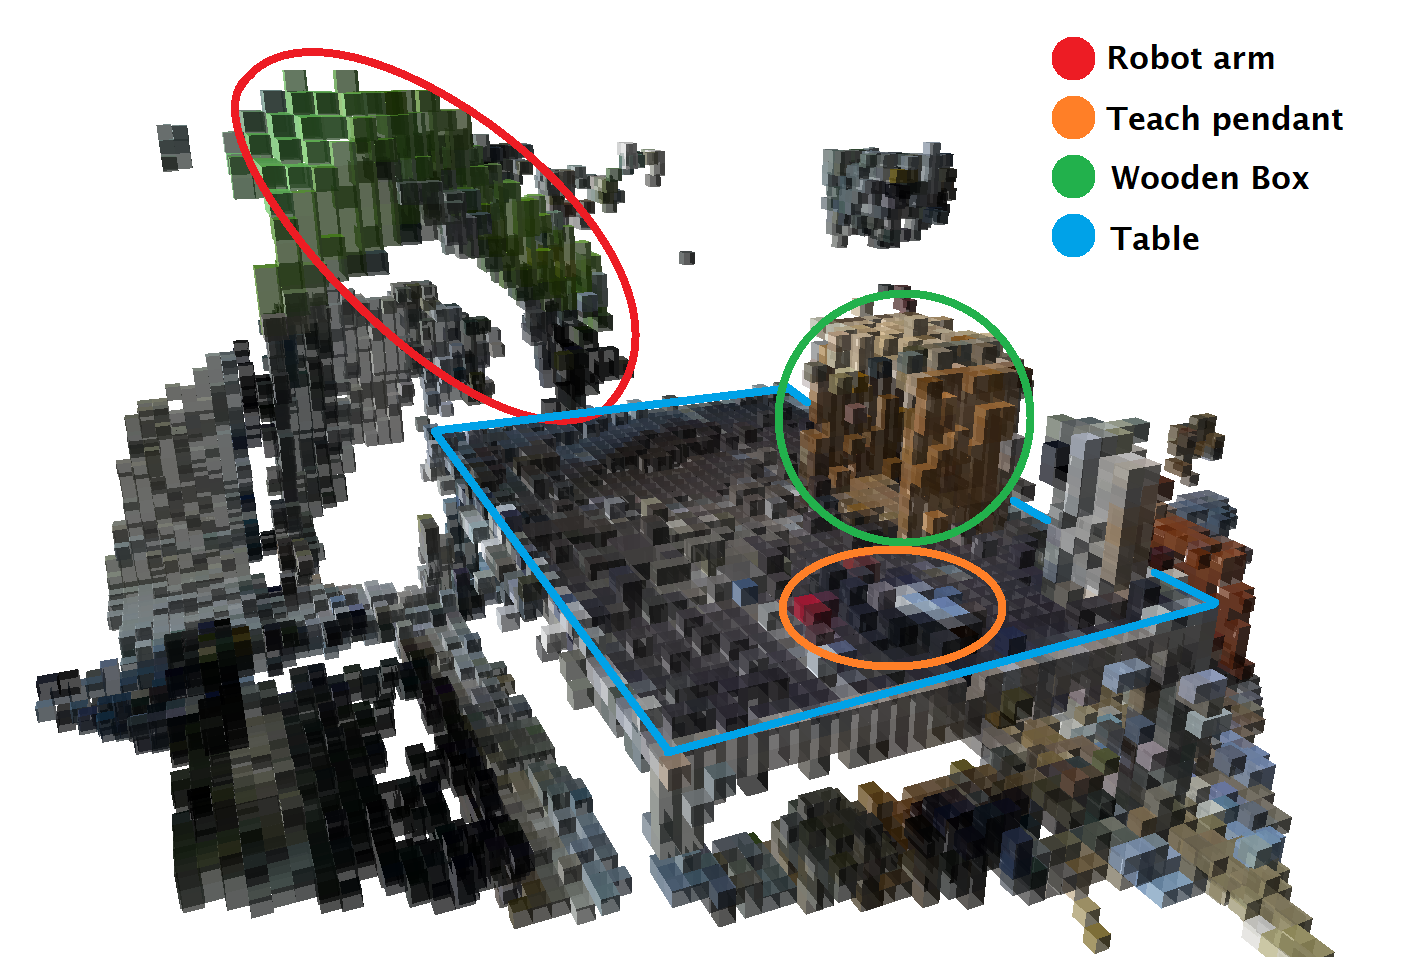
\includegraphics[scale=0.45]{images/occupancy_grid_marked.png}			
	\caption{Generated occupancy grid, already filled with the point cloud data.}
	\label{fig:occupamcy}                      
\end{figure}


\section{Collision avoidance}
\label{sec:avoid}

The collision avoidance also takes place in the \emph{run()} method of the viewer class. A while loop is executed as long as no safe and collision free path is found. Inside this while loop, a line is generated from the current robot position to the position where the robot should move to. The line is generated using the \emph{octomap::ColorOctree.castRay(point3d \&startingpoint, point3d \&direction, point3d \&endpoint, bool ignoreUknownCells, double maxRange )} function.
The starting point is received from the read robot position command. It is important to know that the current position read from the robot is received in millimeters, the unit used for the raycasting in the occupancy grid is meters. Be sure to have the correct units given to the \emph{octomap::ColorOctree.castRay()} function. The direction of the ray can be calculated with simple vector geometrics (\ref{eq:direction}).

\begin{equation}
\label{eq:direction}
	\begin{pmatrix}
	x_{goal}\\
	y_{goal}\\
	z_{goal}
	\end{pmatrix}
	-
	\begin{pmatrix}
	x_{current}\\
	y_{current}\\
	z_{current}
	\end{pmatrix}
	=
		\begin{pmatrix}
	x_{direction}\\
	y_{direction}\\
	z_{direction}
	\end{pmatrix}
\end{equation}

The endpoint returns the center coordinates of the first occupied cell that was hit by the ray. IgnoreUnknownCells defines how unknown cells are treated. For this project, unknown cells are treated as free cells and thus the value needs to be set to true. Since the point cloud data should cover all occupied cells, every other cell should be automatically set to free.
The distance the castRay has to cover can again easily be calculated with vector geometrics (\ref{eq:distance}).

\begin{equation}
\label{eq:distance}
	distance = \sqrt{(x_{goal}-x_{current})^2 + (y_{goal}-y_{current})^2 + (z_{goal}-z_{current})^2}
\end{equation}

The \emph{octomap::ColorOctree.castRay()} function returns a boolean, which is set to true if any occupied cell was hit and the maximum range was not reached. Therefore a true return values represents that an obstacle has been found. If an obstacle is found in the path of the robot, the robt moves a certain distance in z-Direction, in order to try to move over the object. After moving upwards, the castRay() starts again. To avoid reaching positions the robot can't reach, only a certain amount of increments along the z-Axis are done. After five attempts to avoid the obstacle, the program is paused and waits for a user input, approving that the object has been removed from the robot workspace.

Since the robot is captured by the cameras and therefore marked as occupied cells inside the map, any robot movement upwards  would generate a collision with the robot model. To avoid this straight upwards movements do not trigger a raycasting. The same goes for downwards movements when a piece should be picked up. The movement down to the piece would generate a collision with the piece and result in a collision. This means that for the use case created for this project only horizontal movements use the raycasting to detect collisions with objects in the robot workspace. Figure \ref{fig:system} shows a graphical overview on how the collision avoidance system operates.

\newpage
\begin{figure}[H]
	\centering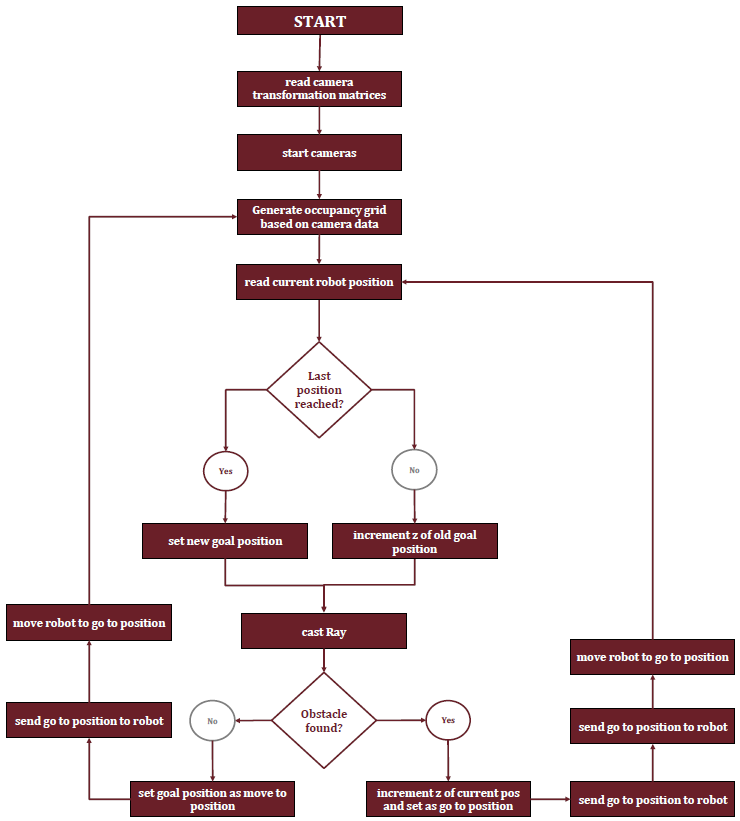
\includegraphics[scale=0.9]{images/system_overview.png}
	\caption{Graphical overview of the collision avoidance system.}
	\label{fig:system}
\end{figure}





\chapter{Results and outlook}
\label{chap:results}

\subsubsection{Robot communication and robot movements} 
A first result was achieved by establishing a communication with the robot. The system is able to read the current cartesian position of the robot and write a new position into the position register of the robot controller. The communication is part of the program which runs on the robot. This program implements a sequential communication which has a strict order which needs to be followed, otherwise the system and the robot will end up not communicating with each other. As a first step to improve the collision avoidance system, a more dynamic communication should be implemented. This could be done by additionally sending communication flags from the system to the robot. These flags could then trigger the read, write or move command.

The robot movements are currently limited to linear movements, since the raycasting of movements from start to endpoint is the limiter. A way to implement joint movements could be, by dividing the joint movements in small fractions, calculate the cartesian positions of each fraction and check for collisions along these fractions before executing the joint movement.

\subsubsection{Cameras and data acquisition}
Currently, the workspace is monitored with two cameras. However, it was revealed that two cameras are not enough because if the robot is positioned in front of a camera a shadow is casted on behind objects and necessary data is lost. To avoid this data loss it is suggested to use more cameras since the infrared structure of each camera interferes with each other. it would be best if each camera can be triggered separately in order to avoid interference. Alternatively a photogrammetry based system could be used to avoid having problems with the IR pattern.  A second problem encountered with the current cameras, is the unstable connection over the USB cable. This was expected since one of the cameras needed a long (5m) cable to reach the computer where the system runs. To avoid having long USB cables, cameras with Ethernet connection are suggested. 

\subsubsection{Point cloud and map generation}
The two cameras deliver a point cloud which reaches all necessary specifications in order to create an occupancy grid. The PCL would have many more functions in order to improve noise reduction and achive a more accurate mapping process. The map currently has the robot model included as occupied cells. This leads to faulty collision predictions with the robot model, especially in movements along the Z-axis. Removing the robot model from the map would solve this problem.

\subsubsection{Collision avoidance}
A simple object detection and collision avoidance was realised using the octomaps raycasting function. Therefore the system is able to detect objects in a straight path of the current position of the robot to its next position. This only regards the tool center point, collisions with any part of the robot body and the object are not detected. In order to have an industrial application it is necessary to implement a collision detection for the whole robot body. This task would need further research.
\chapter{Conclusion}
\label{chap:conclusion}

A basic approach for a collision avoidance system for collaborative robots has been programmed and partially successfully implemented. 

The advantages and disadvantages of necessary tools like cameras and libraries have been evaluated and tested on a basic use case. 
For industrial use a better performing and more extended camera set up needs to be implemented, so the workspace can be monitored adequately.

The open source libraries used for point cloud processing and occupancy grid mapping provide the needed algorithms for this project.

The programmed use case is very basic but enables to create the most common movements of an industrial application and is therefore sufficient for this project. More important is the communication from robot to system and back. The Robots position can be sent to the system and the robots movement can be defined externally and extended with gripping commands.

Besides the movement of the robot, the data gathering of the robots workspace is key in this project. Cameras need to be mounted in the right positions to avoid creating shadows over the obstacles in the workspace and thus preventing them to be detected.





%---------------------------------------------------------------------------

% Selbst�ndigkeitserkl�rung
%---------------------------------------------------------------------------
%\cleardoublepage
\phantomsection 
\addcontentsline{toc}{chapter}{Declaration of authorship}
\chapter*{Declaration of primary authorship}
\label{chap:declaration_authorship}

\vspace*{10mm} 

I hereby confirm that I have written this thesis independently and without using other sources and resources than those specified in the bibliography. All text passages which were not written by me are marked as quotations and provided with the exact indication of its origin. 

\vspace{15mm}

\begin{tabbing}
xxxxxxxxxxxxxxxxxxxxxxxxxxxxxx\=xxxxxxxxxxxxxxxxxxxxxxxxxxxxxx\=xxxxxxxxxxxxxxxxxxxxxxxxxxxxxx\kill
Place, Date:		\> Biel, \versiondate \\ \\ 
Last Name, First Name:	\> Aeschlimann, Dario 	\>  \\ \\ \\ \\ 
Signature:	\> ......................................\> ...................................... \\
\end{tabbing}

%---------------------------------------------------------------------------

% Glossary
%---------------------------------------------------------------------------
%\cleardoublepage
%\phantomsection 
%\addcontentsline{toc}{chapter}{Glossary}
%\renewcommand{\glossaryname}{Glossay}
%\printglossary
%---------------------------------------------------------------------------

% Bibliography
%---------------------------------------------------------------------------
%\cleardoublepage
%\phantomsection 
%\addcontentsline{toc}{chapter}{Bibliography}
\bibliographystyle{IEEEtranS}
\bibliography{database/bibliography}{}
%---------------------------------------------------------------------------

% Listings
%---------------------------------------------------------------------------
%\cleardoublepage
\phantomsection 
\addcontentsline{toc}{chapter}{List of figures}
\listoffigures
%\cleardoublepage
%\phantomsection 
%\addcontentsline{toc}{chapter}{List fo tables}
%\listoftables
\phantomsection 
\addcontentsline{toc}{chapter}{List fo listings}
\lstlistoflistings
%---------------------------------------------------------------------------

% Index
%---------------------------------------------------------------------------
%\cleardoublepage
%\phantomsection 

%\addcontentsline{toc}{chapter}{Index}
%\printindex
%---------------------------------------------------------------------------

% Attachment:
%---------------------------------------------------------------------------
\phantomsection 
\appendix
\clearpage
\pagenumbering{arabic}% resets `page` counter to 1
\renewcommand*{\thepage}{A\arabic{page}}
\settocdepth{section}
\chapter*{Appendices}
\addcontentsline{toc}{chapter}{Appendices}


\chapter{Datasheet Fanuc CR-35iA}
\label{app:datafanuc}
\begin{figure}[b]
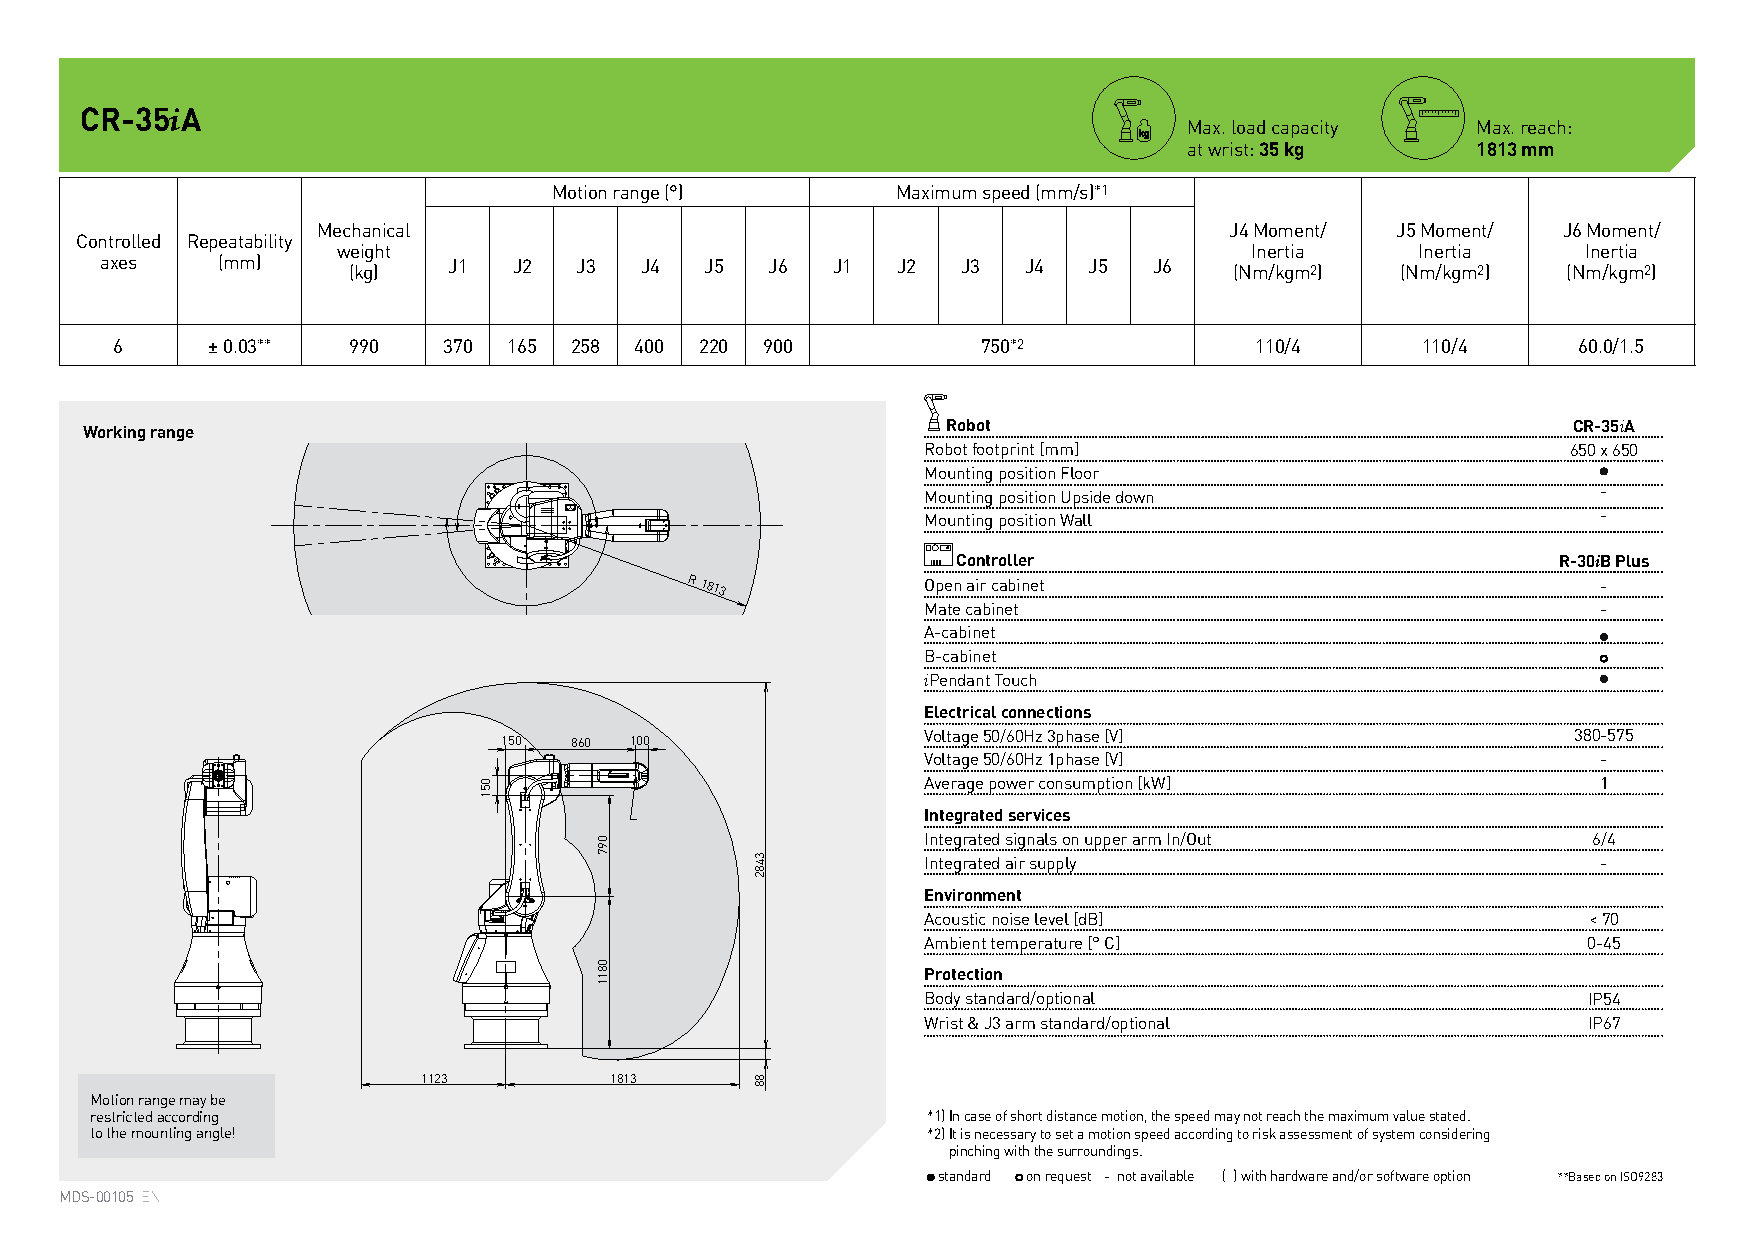
\includepdf[pagecommand={\thispagestyle{plain}}, page={1}]{appendix/datasheet-CR35iA.pdf}
\end{figure}
\chapter{Datasheet Asus Xtion PRO Live}
\label{app:dataasus}
\begin{figure}[b]
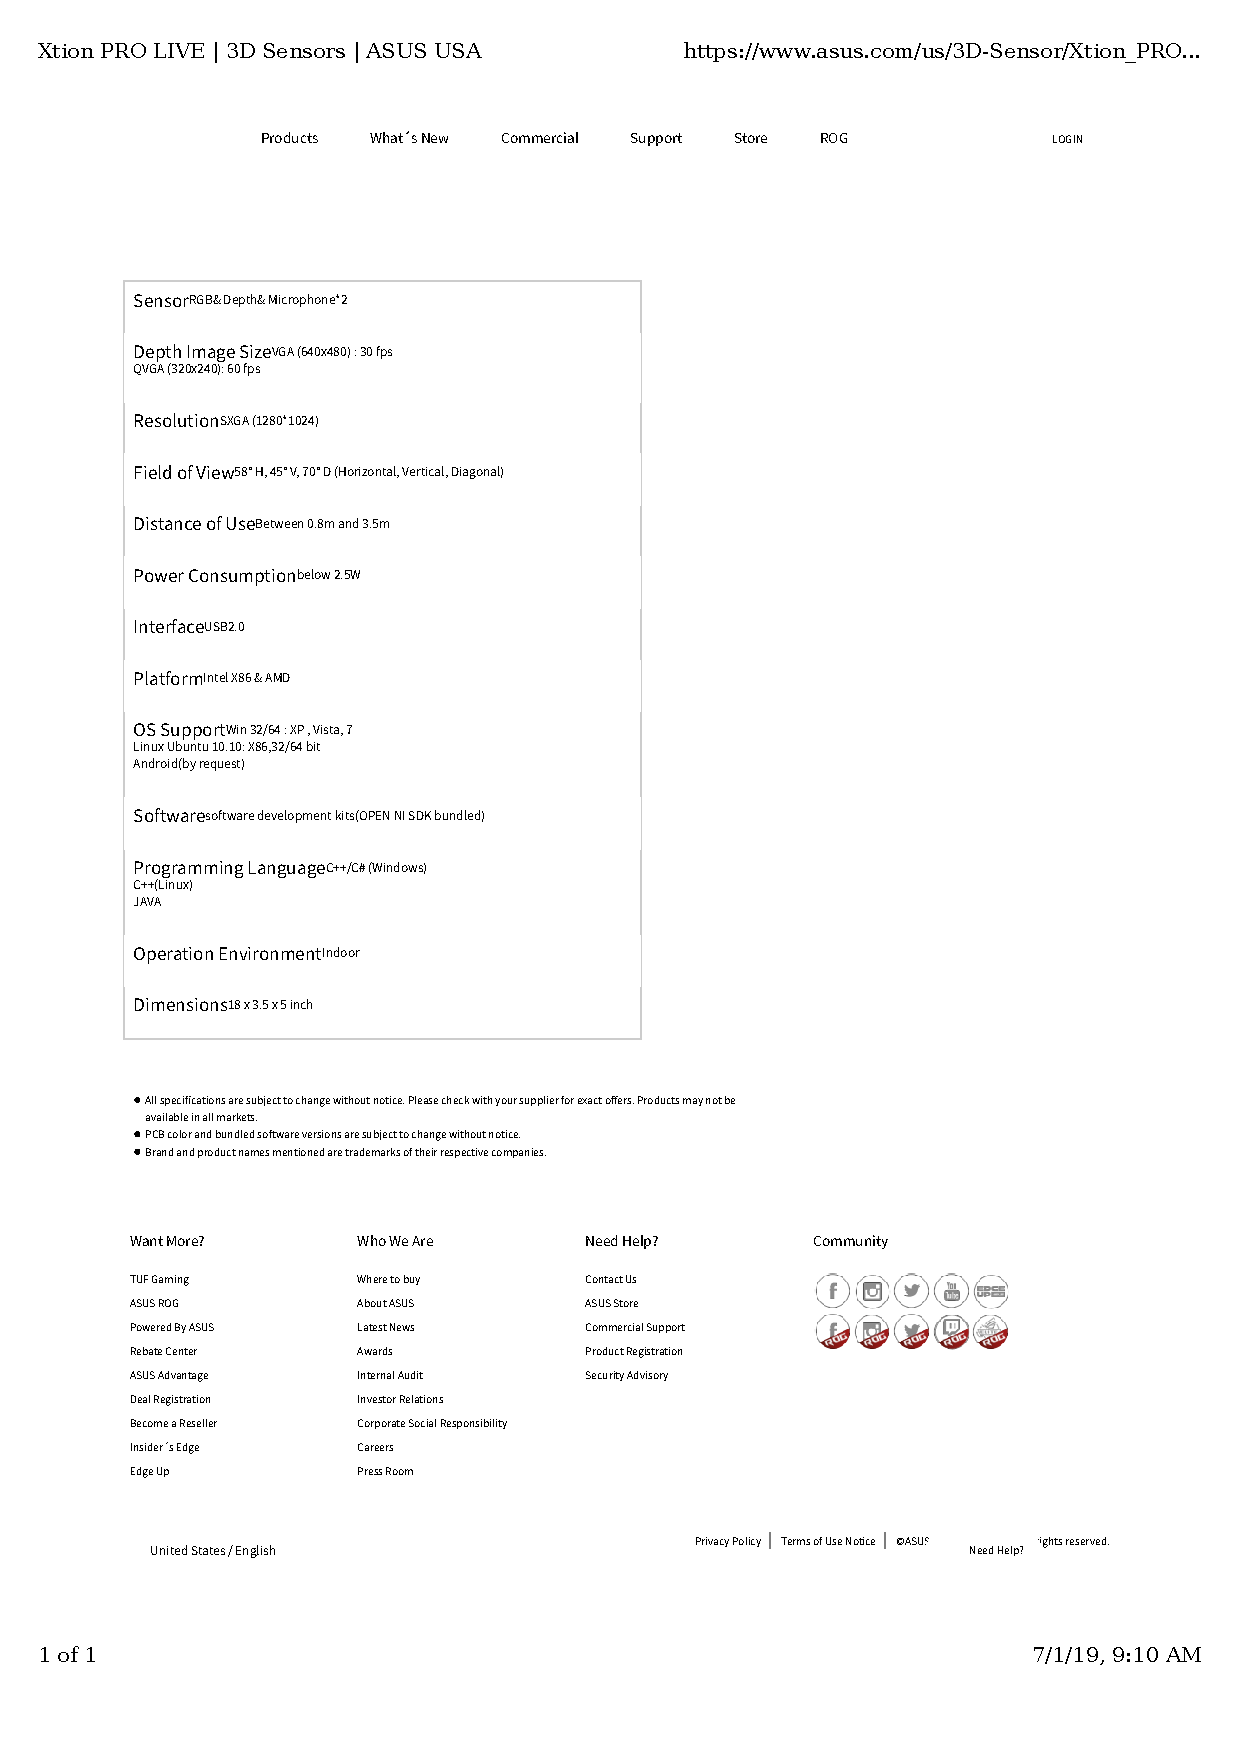
\includepdf[scale=0.75, pagecommand={\thispagestyle{plain}}, page={1}]{appendix/asus_xtion.pdf}
\end{figure}
\lstset{language=Pascal,
	basicstyle=\ttfamily,
	numbers=left,
	stepnumber=1,
	keywordstyle=\color{blue},
	stringstyle=\color{red},
	commentstyle=\color{green},
	morecomment=[l][\color{magenta}]{\#}
}     

\chapter{KAREL Read - code}
\label{app:karelread}
\begin{lstlisting}[frame = single, label={lst:karelread}]  
PROGRAM test_read_c
%STACKSIZE = 4000
%NOLOCKGROUP
%NOPAUSE=ERROR+COMMAND+TPENABLE
%ENVIRONMENT uif
%ENVIRONMENT sysdef
%ENVIRONMENT memo
%ENVIRONMENT kclop
%ENVIRONMENT bynam
%ENVIRONMENT fdev
%ENVIRONMENT flbt
%ENVIRONMENT REGOPE
%INCLUDE klevccdf
%INCLUDE klevkeys
%INCLUDE klevkmsk
----------------------------------------------
VAR
file_var   : FILE
STATUS  : INTEGER
entry   : INTEGER
cur_pos: XYZWPR
c_real_array : ARRAY[6] OF REAL  -- REAL Array
indx   : INTEGER    --for counter

CONST

MOVE_PREG = 90			-- POS Register Number wich will be used to store the JointPos
WRITE_FLAG = 199
READ_FLAG = 200
----------------------------------------------
BEGIN
indx = 1	
FORCE_SPMENU(TP_PANEL,SPI_TPUSER,1)
WRITE TPDISPLAY (CHR(128),CHR(137))
SET_FILE_ATR(file_var, ATR_IA)
-- set the server port before doing a connect
SET_VAR(entry, '*SYSTEM*','$HOSTS_CFG[3].$SERVER_PORT',59004,STATUS)
WRITE TPDISPLAY('Connecting..',CR)
MSG_CONNECT('S3:',STATUS)
WRITE TPDISPLAY(' CONNECT STATUS = ',STATUS,CR)
IF STATUS = 0 THEN
-- Open S3:
WRITE TPDISPLAY('Opening',CR)
--   FOR tmp_int1 = 1 TO 20 DO
OPEN FILE file_var ('rw','S3:')
STATUS = IO_STATUS(file_var)
WRITE TPDISPLAY(STATUS,CR)
IF STATUS = 0 THEN
-- write an integer
WRITE TPDISPLAY('Reading',CR)
cur_pos = CURPOS(0,0)
WRITE TPDISPLAY('Cartesian Positions:', cur_pos, CR)
c_real_array[1] = cur_pos.X
WRITE TPDISPLAY('X =', cur_pos.X , CR)
WRITE TPDISPLAY('realX =', c_real_array[1] , CR)

c_real_array[2] = cur_pos.Y
WRITE TPDISPLAY('Y =', cur_pos.Y , CR)
WRITE TPDISPLAY('realY =', c_real_array[2] , CR)

c_real_array[3] = cur_pos.Z
WRITE TPDISPLAY('Z =', cur_pos.Z , CR)
WRITE TPDISPLAY('realZ =', c_real_array[3] , CR)

c_real_array[4] = cur_pos.W
WRITE TPDISPLAY('W =', cur_pos.W , CR)


c_real_array[5] = cur_pos.P
WRITE TPDISPLAY('P =', cur_pos.P , CR)

c_real_array[6] = cur_pos.R
WRITE TPDISPLAY('R =', cur_pos.R , CR)


FOR indx = 1 TO 6 DO
--WRITE TPDISPLAY('send jpos real array[',indx,']:', CR)
--WRITE TPDISPLAY(c_real_array[indx], CR)
WRITE file_var(c_real_array[indx], CR)
ENDFOR


CLOSE FILE file_var
ENDIF
--ENDFOR
WRITE TPDISPLAY('Disconnecting..',CR)
MSG_DISCO('S3:',STATUS)
WRITE TPDISPLAY('Done.',CR)
SET_INT_REG(WRITE_FLAG, 1, STATUS)
SET_INT_REG(READ_FLAG, 0, STATUS)
ENDIF
END test_read_c
\end{lstlisting}
\lstset{language=Pascal,
	basicstyle=\ttfamily,
	numbers=left,
	stepnumber=1,
	keywordstyle=\color{blue},
	stringstyle=\color{red},
	commentstyle=\color{green},
	morecomment=[l][\color{magenta}]{\#}
}     

\chapter{KAREL Write - code}
\label{app:karelwrite}
\begin{lstlisting}[frame = single, label={lst:karelread}]  
PROGRAM test_write_c
%STACKSIZE = 4000
%NOLOCKGROUP
%NOPAUSE=ERROR+COMMAND+TPENABLE
%ENVIRONMENT uif
%ENVIRONMENT sysdef
%ENVIRONMENT memo
%ENVIRONMENT kclop
%ENVIRONMENT bynam
%ENVIRONMENT fdev
%ENVIRONMENT flbt
%ENVIRONMENT REGOPE
%INCLUDE klevccdf
%INCLUDE klevkeys
%INCLUDE klevkmsk
-------------------------------------------------------------------------------
VAR
file_var   : FILE
tmp_int   : INTEGER
tmp_int1  : INTEGER
tmp_str   : STRING[128]
STATUS  : INTEGER
entry   : INTEGER
n_j_pos : JOINTPOS6     -- position of robot joints to go to, IMPORTANT: JOINTPOSX must be defined, just using JOINTPOS results in uninitialized variable error. X marks the number of Joints.
new_pos : XYZWPR
stat_   : INTEGER     -- status variable
n_real_array : ARRAY[6] OF REAL  -- REAL Array
indx   : INTEGER    --for counter
group_no: INTEGER
CONST

MOVE_PREG = 90			-- POS Register Number wich will be used to store the JointPos
WRITE_FLAG = 199
READ_FLAG = 200
-------------------------------------------------------------------------------
BEGIN
group_no = 1
--Setze $UTOOL $UFRAME mit aktuell im TP eingestellten UT und UF
$GROUP[group_no].$UFRAME = $MNUFRAME[group_no, $MNUFRAMENUM[group_no]]
$GROUP[group_no].$UTOOL = $MNUTOOL[group_no, $MNUTOOLNUM[group_no]]
new_pos = CURPOS(0,0)
--SET_POS_REG(MOVE_PREG, new_pos, STATUS)
FORCE_SPMENU(TP_PANEL,SPI_TPUSER,1)
WRITE TPDISPLAY (CHR(128),CHR(137))
SET_FILE_ATR(file_var, ATR_IA)
-- set the server port before doing a connect
SET_VAR(entry, '*SYSTEM*','$HOSTS_CFG[4].$SERVER_PORT',59003,STATUS)
WRITE TPDISPLAY('Connecting..',CR)
MSG_CONNECT('S4:',STATUS)
WRITE TPDISPLAY(' CONNECT STATUS = ',STATUS,CR)
IF STATUS = 0 THEN
-- Open S4:
WRITE TPDISPLAY('Opening',CR)
--   FOR tmp_int1 = 1 TO 20 DO
OPEN FILE file_var ('rw','S4:')
STATUS = IO_STATUS(file_var)
WRITE TPDISPLAY(STATUS,CR)
IF STATUS = 0 THEN
-- write an integer
WRITE TPDISPLAY('Reading',CR)

-- Read 10 bytes

FOR indx = 1 TO 6 DO
BYTES_AHEAD(file_var, entry, STATUS)
READ file_var (tmp_str::126)
WRITE TPDISPLAY('receive:',tmp_str,CR )
CNV_STR_REAL(tmp_str, n_real_array[indx])
--              n_real_array[indx] = tmp_str
--		READ file_var (n_real_array[indx]::126,CR)
WRITE TPDISPLAY('2.receive:',n_real_array[indx],CR )
ENDFOR
new_pos.X = n_real_array[1]
new_pos.Y = n_real_array[2]
new_pos.Z = n_real_array[3]
new_pos.W = n_real_array[4]
new_pos.P = n_real_array[5]
new_pos.R = n_real_array[6]
WRITE TPDISPLAY('New Positions:',new_pos, CR)
SET_POS_REG(MOVE_PREG, new_pos, STATUS)

CLOSE FILE file_var
ENDIF

WRITE TPDISPLAY('Disconnecting..',CR)
MSG_DISCO('S4:',STATUS)
WRITE TPDISPLAY('Done.',CR)
SET_INT_REG(WRITE_FLAG, 0, STATUS)
SET_INT_REG(READ_FLAG, 0, STATUS)
ENDIF
END test_write_c
\end{lstlisting}
\chapter{C++ com\_func.h \- code}
\label{app:com_func.h}

\lstset{language=C++,
	numbers=left,
	stepnumber=1,
	basicstyle=\ttfamily,
	keywordstyle=\color{blue},
	stringstyle=\color{red},
	commentstyle=\color{green},
	morecomment=[l][\color{magenta}]{\#}
}

\begin{lstlisting}[frame = single, label={lst:cppread1}]
#ifndef COM_FUNC_H
#define COM_FUNC_H

#define MAXLINE 512

#define SERV_TCP_PORT_READ 59004
#define SERV_TCP_PORT_WRITE 59003

//#define SERV_HOST_ADDR "147.87.149.40" /* RoboGuide PC Robot */
#define SERV_HOST_ADDR "147.87.144.251" /* Robot */




/**
 * @brief connectReadJoint
 * @param current_joint_pos
 * @return
 */
float* connectReadJoint (float *current_joint_pos);

/**
 * @brief connectReadCartesian
 * @param current_cartesian_pos
 * @return
 */
float *connectReadCartesian (float *current_cartesian_pos);

/**
 * @brief connectWriteJoint
 * @param goto_joint_pos
 * @param current_joint_pos
 */
void connectWriteJoint (float *goto_joint_pos, float *current_joint_pos);

/**
 * @brief connectWriteCartesian
 * @param goto_cartesian_pos
 * @param current_cartesian_pos
 */
void connectWriteCartesian (float *goto_cartesian_pos, float *current_cartesian_pos);

/**
 * @brief readJointPos
 * @param sockfd
 * @return
 */
float* readPos(int sockfd);

/**
 * @brief writeJointPos
 * @param sockfd
 * @param goto_pos
 */
void writePos (int sockfd, float *goto_pos);

/**
 * @brief readline
 * @param fd
 * @param ptr
 * @param maxlen
 * @param input
 * @return
 */
float readline(int fd, char *ptr, int maxlen, char input[MAXLINE+1]);

/**
 * @brief written
 * @param fd
 * @param ptr
 * @param nbytes
 * @return
 */
int written(int fd, char *ptr, int nbytes);

/**
 * @brief gripperOn
 */
void gripperOn (void);

/**
 * @brief gripperOff
 */
void gripperOff (void);

#endif // COM_FUNC_H
\end{lstlisting}

\chapter{C++ com\_func.cpp - code}
\label{app:com_func.cpp}

\lstset{language=C++,
	numbers=left,
	stepnumber=1,
	basicstyle=\ttfamily,
	keywordstyle=\color{blue},
	stringstyle=\color{red},
	commentstyle=\color{green},
	morecomment=[l][\color{magenta}]{\#}
}

\begin{lstlisting}[frame = single, label={lst:cppread1}]
#include <unistd.h>
#include <stdio.h>
#include <sys/types.h>
#include <sys/socket.h>
#include <netinet/in.h>
#include <arpa/inet.h>
#include <cstring>
#include <iostream>
#include <stdlib.h>
#include <string>
#include <chrono>

#include "com_func.h"
using namespace std;

float *connectReadJoint (float *current_joint_pos){
// READ SETUP

int sockfd;
struct sockaddr_in serv_addr_read;
bzero((char *) &serv_addr_read, sizeof(serv_addr_read));
serv_addr_read.sin_family = AF_INET;
serv_addr_read.sin_addr.s_addr = inet_addr(SERV_HOST_ADDR);
serv_addr_read.sin_port = htons(SERV_TCP_PORT_READ);

// READ JOINT POS

if((sockfd = socket(AF_INET, SOCK_STREAM,0)) < 0){
printf("Client: Can't Open Stream Socket\n");
}
printf("Client: Connecting to READ server...\n");
if(connect(sockfd,(struct sockaddr *) &serv_addr_read, sizeof(serv_addr_read))<0){
printf("Client: Can't Connect to the READ server\n");
}
else{
printf("Client: Connected!\n");
current_joint_pos = readPos(sockfd);
for(int k = 0; k < 6; k++){
printf("joint %d pos: %f \n", k+1, current_joint_pos[k]);
}
}
return current_joint_pos;
}

float *connectReadCartesian (float *current_cartesian_pos){
//    auto startReadConnect = chrono::steady_clock::now();
// READ SETUP
int sockfd;
struct sockaddr_in serv_addr_read;
bzero((char *) &serv_addr_read, sizeof(serv_addr_read));
serv_addr_read.sin_family = AF_INET;
serv_addr_read.sin_addr.s_addr = inet_addr(SERV_HOST_ADDR);
serv_addr_read.sin_port = htons(SERV_TCP_PORT_READ);

// READ JOINT POS

if((sockfd = socket(AF_INET, SOCK_STREAM,0)) < 0){
printf("Client: Can't Open Stream Socket\n");
}
printf("Client: Connecting to READ server...\n");
while(connect(sockfd,(struct sockaddr *) &serv_addr_read, sizeof(serv_addr_read))<0){
printf("Client: Can't Connect to the READ server\r");
}

printf("Client: Connected!\n");
current_cartesian_pos = readPos(sockfd);
printf("X pos: %f \n", current_cartesian_pos[0]);
printf("Y pos: %f \n", current_cartesian_pos[1]);
printf("Z pos: %f \n", current_cartesian_pos[2]);
printf("W pos: %f \n", current_cartesian_pos[3]);
printf("P pos: %f \n", current_cartesian_pos[4]);
printf("R pos: %f \n", current_cartesian_pos[5]);


//    auto endReadConnect = chrono::steady_clock::now();
//    cout << "Elapsed Time in milliseconds (connect read): " << chrono::duration_cast<chrono::milliseconds>(endReadConnect - startReadConnect).count() << "ms" << endl;
return current_cartesian_pos;
}

void connectWriteJoint (float *goto_joint_pos, float *current_joint_pos){
//WRITE SETUP
int sockfd_write;
struct sockaddr_in serv_addr_write;
bzero((char *) &serv_addr_write, sizeof(serv_addr_write));
serv_addr_write.sin_family = AF_INET;
serv_addr_write.sin_addr.s_addr = inet_addr(SERV_HOST_ADDR);
serv_addr_write.sin_port = htons(SERV_TCP_PORT_WRITE);

// WRITE JOINT POS
if((sockfd_write = socket(AF_INET, SOCK_STREAM,0)) < 0){
printf("Client: Can't Open Stream Socket\n");
}
printf("Client: Connecting to WRITE server...\n");
if(connect(sockfd_write,(struct sockaddr *) &serv_addr_write, sizeof(serv_addr_write))<0){
printf("Client: Can't Connect to the WRITE server\n");
}
else{
for(int s = 0; s < 6; s++){
goto_joint_pos[s] = current_joint_pos[s] + 10.0f;
printf("future joint %d pos: %f \n", s+1, goto_joint_pos[s]);
}
writePos(sockfd_write, goto_joint_pos);
}
}

void connectWriteCartesian (float *goto_cartesian_pos, float *current_cartesian_pos){
//    auto startWriteConnect = chrono::steady_clock::now();
//WRITE SETUP
int sockfd_write;
struct sockaddr_in serv_addr_write;
bzero((char *) &serv_addr_write, sizeof(serv_addr_write));
serv_addr_write.sin_family = AF_INET;
serv_addr_write.sin_addr.s_addr = inet_addr(SERV_HOST_ADDR);
serv_addr_write.sin_port = htons(SERV_TCP_PORT_WRITE);

// WRITE JOINT POS
if((sockfd_write = socket(AF_INET, SOCK_STREAM,0)) < 0){
printf("Client: Can't Open Stream Socket\n");
}
printf("Client: Connecting to WRITE server...\n");
while(connect(sockfd_write,(struct sockaddr *) &serv_addr_write, sizeof(serv_addr_write))<0){
printf("Client: Can't Connect to the WRITE server\r");
}
printf("Client: Connected!\n");

printf("future X pos: %f \n", goto_cartesian_pos[0]);
printf("future Y pos: %f \n", goto_cartesian_pos[1]);
printf("future Z pos: %f \n", goto_cartesian_pos[2]);
printf("future W pos: %f \n", goto_cartesian_pos[3]);
printf("future P pos: %f \n", goto_cartesian_pos[4]);
printf("future R pos: %f \n", goto_cartesian_pos[5]);
writePos(sockfd_write, goto_cartesian_pos);
//    auto endWriteConnect = chrono::steady_clock::now();
//    cout << "Elapsed Time in milliseconds (connect write): " << chrono::duration_cast<chrono::milliseconds>(endWriteConnect - startWriteConnect).count() << "ms" << endl;

}


float * readPos (int sockfd)
{
//    printf("Reading current joint positions...\n");
char input[MAXLINE+1];
static float input_float[6];
char recvline[MAXLINE + 1];
for(int x=0; x < 6; x++)
{
//memset (input_float, 0, 6);
memset (input, 0, MAXLINE+1);
input_float[x] = readline(sockfd, recvline, 126, input);
}
return input_float;
}

void writePos (int sockfd, float *goto_pos)
{
char sendline[MAXLINE];
for(int y=0; y < 6; y++)
{
sprintf(sendline, "%f", goto_pos[y]);
//        printf("sendline %u : %s\n", y, sendline);

if(written(sockfd, sendline, 126)!=126){
printf("writeJointPos:written error on sock\n");
}
//        sleep(1);
}
}

float readline(int fd, char *ptr, int maxlen, char input[MAXLINE+1])
{
int n, rc;
char c;
for(n = 0; n < maxlen; n++){
if((rc = read(fd, &c, 1)) == 1){
input[n] = c;
*ptr++ = c;
if(c=='\n'){
break;
}
else if(rc== 0) {
if(n== 0) {
return (0);
}
else{

break;
}
}
}
else{
return (-1);
}
}
float f = atof(input);
*ptr = 0;
return (f);
}

int written(int fd, char *ptr, int nbytes)
{
int nleft, nwritten;
nleft = nbytes;
//    printf("Client: nleft size: %d \n", nleft);
while(nleft > 0) {
//        printf("Client: while write started\n");
nwritten = write(fd, ptr, nleft); /*was nleft*/
//        printf("Client: nwritten size: %d \n", nwritten);
//        printf("Client: write command executed!\n");
if(nwritten <= 0) {
//            printf("Client: return nwritten\n");
return(nwritten);
}
//        printf("Client: nleft and ptr\n");
nleft -= nwritten;
//        printf("Client: nleft size: %d \n", nleft);
ptr += nwritten;
}
//    printf("Client: return nbytes - nleft: %d \n", nbytes-nleft);
return(nbytes - nleft);
}


void gripperOn (void){
system("lua5.3 ../Rob195/1.txt");
}

void gripperOff (void){
system("lua5.3 ../Rob195/0.txt");
}

\end{lstlisting}
\chapter{C++ main.cpp - code}
\label{app:main.cpp}

\lstset{language=C++,
	numbers=left,
	stepnumber=1,
	basicstyle=\ttfamily,
	keywordstyle=\color{blue},
	stringstyle=\color{red},
	commentstyle=\color{green},
	morecomment=[l][\color{magenta}]{\#}
}

\begin{lstlisting}[frame = single, label={lst:cppread1}]
#include <unistd.h>
#include <stdio.h>
#include <sys/types.h>
#include <sys/socket.h>
#include <netinet/in.h>
#include <arpa/inet.h>
#include <cstring>
#include <iostream>
#include <stdlib.h>
#include <string>
#include <math.h>
#include <chrono>

#include <pcl/io/openni2_grabber.h>
#include <pcl/visualization/cloud_viewer.h>
#include <pcl/io/pcd_io.h>
#include <pcl/io/png_io.h>
#include <pcl/io/ply_io.h>
#include <pcl/point_types.h>
#include <pcl/console/parse.h>
#include <pcl/common/transforms.h>
#include <pcl/point_types.h>
#include <pcl/filters/passthrough.h>
#include <pcl/compression/octree_pointcloud_compression.h>
#include <pcl/filters/voxel_grid.h>

#include <octomap/octomap.h>
#include <octomap/ColorOcTree.h>

#include "com_func.h"

#define SERV_TCP_PORT_READ 59004
#define SERV_TCP_PORT_WRITE 59003


using namespace std;
using namespace pcl;

pcl::PointCloud<pcl::PointXYZRGBA>::Ptr transformedCloudCamB (new pcl::PointCloud<pcl::PointXYZRGBA> ());
pcl::PointCloud<pcl::PointXYZRGBA>::Ptr transformedCloudCamA (new pcl::PointCloud<pcl::PointXYZRGBA> ());
pcl::io::OctreePointCloudCompression<pcl::PointXYZRGBA>* PointCloudEncoder;
pcl::io::OctreePointCloudCompression<pcl::PointXYZRGBA>* PointCloudDecoder;
octomap::ColorOcTree rayMap(0.04);

int nrows = 4;
int ncols = 4;

Eigen::Matrix4f transformCamA = Eigen::Matrix4f::Zero(nrows,ncols);
Eigen::Matrix4f transformCamB = Eigen::Matrix4f::Zero(nrows,ncols);

int positionIndex = 0;
bool debug = false;
bool rayMapinit = false;



class SimpleOpenNIViewer
{
public:
SimpleOpenNIViewer () : viewer ("PCL OpenNI Viewer") {}
void cloud_cb_2_ (const pcl::PointCloud<pcl::PointXYZRGBA>::ConstPtr &cloud)
{
if (!viewer.wasStopped()){
//            auto startPCgenCamB = chrono::steady_clock::now();
// Create the filtering object
pcl::PassThrough<pcl::PointXYZRGBA> pass;

// read cloud transformation data from file
//            cout << "transformCamB = " << endl << transformCamB << endl;


pcl::PointCloud<pcl::PointXYZRGBA>::Ptr CloudCamBfiltered (new pcl::PointCloud<pcl::PointXYZRGBA> ());
pcl::PointCloud<pcl::PointXYZRGBA>::Ptr CloudCamBVoxelGrid (new pcl::PointCloud<pcl::PointXYZRGBA> ());

pass.setInputCloud (cloud);
pass.setFilterFieldName ("z");
pass.setFilterLimits (0.0, 3.5);
//pass.setFilterLimitsNegative (true);
pass.filter (*CloudCamBfiltered);

pcl::VoxelGrid<pcl::PointXYZRGBA> voxelFilter;
voxelFilter.setInputCloud(CloudCamBfiltered);
voxelFilter.setLeafSize (0.01f, 0.01f, 0.01f);
voxelFilter.filter (*CloudCamBVoxelGrid);

// Executing the transformation
pcl::transformPointCloud (*CloudCamBVoxelGrid, *transformedCloudCamB, transformCamB);

//    (row, column)
viewer.showCloud (transformedCloudCamB, cloudnameB);
//            if(debug == true){
stringstream stream;
stream << "inputCloudCamB.pcd";
string filename = stream.str();
io::savePCDFileASCII(filename, *CloudCamBfiltered);
//            PCL_ERROR("Problem saving %s.\n", filename.c_str());
stream.str(std::string());
stream << "transformedCloudB.pcd";
filename = stream.str();
io::savePCDFileASCII(filename, *transformedCloudCamB);
stream.str(std::string());
stream << "inputCLoudCamB.png";
filename = stream.str();
io::savePNGFile(filename, *cloud, "rgb");
//            cout<< "Saved " << filename << "." << endl;
//            cloud = transformedCloudCamB;
//            }
//            auto endPCgenCamB = chrono::steady_clock::now();
//            cout << "Elapsed Time in milliseconds (camB PointCloud generation): " << chrono::duration_cast<chrono::milliseconds>(endPCgenCamB - startPCgenCamB).count() << "ms" << endl;
}
}

void cloud_cb_ (const pcl::PointCloud<pcl::PointXYZRGBA>::ConstPtr &cloud)
{
if (!viewer.wasStopped()){
//            auto startPCgenCamA = chrono::steady_clock::now();
// Create the filtering object
pcl::PassThrough<pcl::PointXYZRGBA> pass;

//            cout << "transformCamA = " << endl << transformCamA << endl;

pcl::PointCloud<pcl::PointXYZRGBA>::Ptr CloudCamAfiltered (new pcl::PointCloud<pcl::PointXYZRGBA> ());
pcl::PointCloud<pcl::PointXYZRGBA>::Ptr CloudCamAVoxelGrid (new pcl::PointCloud<pcl::PointXYZRGBA> ());

pass.setInputCloud (cloud);
pass.setFilterFieldName ("z");
pass.setFilterLimits (0.0, 4.1);
//pass.setFilterLimitsNegative (true);
pass.filter (*CloudCamAfiltered);


pcl::VoxelGrid<pcl::PointXYZRGBA> voxelFilter;
voxelFilter.setInputCloud(CloudCamAfiltered);
voxelFilter.setLeafSize (0.01f, 0.01f, 0.01f);
voxelFilter.filter (*CloudCamAVoxelGrid);


// Executing the transformation
pcl::transformPointCloud (*CloudCamAVoxelGrid, *transformedCloudCamA, transformCamA);

//    (row, column)
viewer.showCloud (transformedCloudCamA, cloudnameA);
//            if(debug == true){
stringstream stream;
stream << "inputCloudCamA.pcd";
string filename = stream.str();
io::savePCDFileASCII(filename, *CloudCamAVoxelGrid);
//            PCL_ERROR("Problem saving %s.\n", filename.c_str());
stream.str(std::string());
stream << "transformedCloudA.pcd";
filename = stream.str();
io::savePCDFileASCII(filename, *transformedCloudCamA);
stream.str(std::string());
stream << "inputCLoudCamA.png";
filename = stream.str();
io::savePNGFile(filename, *cloud, "rgb");
//            cout<< "Saved " << filename << "." << endl;
//            cloud = transformedCloudCamA;
//            }
//            auto endPCgenCamA = chrono::steady_clock::now();
//           cout << "Elapsed Time in milliseconds (camA PointCloud generation): " << chrono::duration_cast<chrono::milliseconds>(endPCgenCamA - startPCgenCamA).count() << "ms" << endl;
}
}

void run ()
{
//        //**********************************
//        start first Xtion
Grabber* interface = new io::OpenNI2Grabber("#1");

boost::function<void (const pcl::PointCloud<pcl::PointXYZRGBA>::ConstPtr&)> f =
boost::bind (&SimpleOpenNIViewer::cloud_cb_, this, _1);

interface->registerCallback (f);
interface->start();
//**********************************

//**********************************
//        start second Xtion
pcl::Grabber* interface2 = new io::OpenNI2Grabber("#2");
boost::function<void (const pcl::PointCloud<pcl::PointXYZRGBA>::ConstPtr&)> f2 =
boost::bind (&SimpleOpenNIViewer::cloud_cb_2_, this, _1);

interface2->registerCallback (f2);

interface2->start();
//**********************************

while (!viewer.wasStopped())
{
bool showStatistics = true;
bool reset = false;

pcl::io::compression_Profiles_e compressionProfile = pcl::io::MED_RES_ONLINE_COMPRESSION_WITH_COLOR;

PointCloudEncoder = new pcl::io::OctreePointCloudCompression<pcl::PointXYZRGBA> (compressionProfile, showStatistics);
PointCloudDecoder = new pcl::io::OctreePointCloudCompression<pcl::PointXYZRGBA> ();


pcl::PointCloud<pcl::PointXYZRGBA>::Ptr concatenatedCloud (new pcl::PointCloud<pcl::PointXYZRGBA> ());
pcl::PointCloud<pcl::PointXYZRGBA>::Ptr cloud_filtered (new pcl::PointCloud<pcl::PointXYZRGBA> ());

*concatenatedCloud = *transformedCloudCamA;
*concatenatedCloud += *transformedCloudCamB;

io::savePCDFileASCII("concatenated.pcd", *concatenatedCloud);

pcl::VoxelGrid<pcl::PointXYZRGBA> voxelFilter;
voxelFilter.setInputCloud(concatenatedCloud);
voxelFilter.setLeafSize (0.04f, 0.04f, 0.04f);
voxelFilter.filter (*cloud_filtered);


io::savePCDFileASCII("cloud_filtered.pcd", *cloud_filtered);

// stringstream to store compressed point cloud
std::stringstream compressedData;

// compress point cloud
PointCloudEncoder->encodePointCloud (cloud_filtered, compressedData);

//octomap
//            cout<<"copy data into octomap..."<<endl;
//
//            auto startOctreeGen = chrono::steady_clock::now();
octomap::ColorOcTree tree( 0.04 );
for (float x = -2.5; x <= 2.5; x += 0.08f) {
for (float y = 0; y <= 4; y += 0.08f) {
for (float z = -1.5; z <= 2; z += 0.08f) {
octomap::point3d endpoint(x, y, z);
tree.updateNode(endpoint, false); // integrate 'free' measurement
//                        rayMap.updateNode(endpoint, false);
}
}
}

for (auto p:cloud_filtered->points)
{
tree.updateNode(octomap::point3d(p.x, p.y, p.z), true);
if(rayMapinit == false){
rayMap.updateNode(octomap::point3d(p.x, p.y, p.z), true);
}
}


for (auto p:cloud_filtered->points)
{
tree.integrateNodeColor( p.x, p.y, p.z, p.r, p.g, p.b );
if(rayMapinit == false){
rayMap.integrateNodeColor( p.x, p.y, p.z, p.r, p.g, p.b );
}
}
rayMapinit = true;
//            auto endOctreeGen = chrono::steady_clock::now();
//            cout << "Elapsed Time in milliseconds (Octomap generation): " << chrono::duration_cast<chrono::milliseconds>(endOctreeGen - startOctreeGen).count() << "ms" << endl;

float fixedPos[24][6];
//position 1 left side top 1
fixedPos[0][0] = -860;
fixedPos[0][1] = 1330;
fixedPos[0][2] = -560;
fixedPos[0][3] = 180;
fixedPos[0][4] = 0.0;
fixedPos[0][5] = 90.0;

//position 2 left side bottom
fixedPos[1][0] = -860;
fixedPos[1][1] = 1330;
fixedPos[1][2] = -650;
fixedPos[1][3] = 180;
fixedPos[1][4] = 0.0;
fixedPos[1][5] = 90.0;

//position 3 left side top 2
fixedPos[2][0] = -860;
fixedPos[2][1] = 1330;
fixedPos[2][2] = -560;
fixedPos[2][3] = 180;
fixedPos[2][4] = 0.0;
fixedPos[2][5] = 90.0;

//position 4 right side top 1
fixedPos[3][0] = 600;
fixedPos[3][1] = 1550;
fixedPos[3][2] = -560;
fixedPos[3][3] = 180;
fixedPos[3][4] = 0.0;
fixedPos[3][5] = 90.0;

//position 5 right side bottom
fixedPos[4][0] = 600;
fixedPos[4][1] = 1550;
fixedPos[4][2] = -655;
fixedPos[4][3] = 180;
fixedPos[4][4] = 0.0;
fixedPos[4][5] = 90.0;

//position 6 right side top 2
fixedPos[5][0] = 600;
fixedPos[5][1] = 1550;
fixedPos[5][2] = -560;
fixedPos[5][3] = 180;
fixedPos[5][4] = 0.0;
fixedPos[5][5] = 90.0;

//position 7 left side top 1
fixedPos[6][0] = -860;
fixedPos[6][1] = 1550;
fixedPos[6][2] = -560;
fixedPos[6][3] = 180;
fixedPos[6][4] = 0.0;
fixedPos[6][5] = 90.0;

//position 8 left side bottom
fixedPos[7][0] = -860;
fixedPos[7][1] = 1550;
fixedPos[7][2] = -650;
fixedPos[7][3] = 180;
fixedPos[7][4] = 0.0;
fixedPos[7][5] = 90.0;

//position 9 left side top 2
fixedPos[8][0] = -860;
fixedPos[8][1] = 1550;
fixedPos[8][2] = -560;
fixedPos[8][3] = 180;
fixedPos[8][4] = 0.0;
fixedPos[8][5] = 90.0;

//position 10 right side top 1
fixedPos[9][0] = 600;
fixedPos[9][1] = 1330;
fixedPos[9][2] = -560;
fixedPos[9][3] = 180;
fixedPos[9][4] = 0.0;
fixedPos[9][5] = 90.0;

//position 11 right side bottom
fixedPos[10][0] = 600;
fixedPos[10][1] = 1330;
fixedPos[10][2] = -655;
fixedPos[10][3] = 180;
fixedPos[10][4] = 0.0;
fixedPos[10][5] = 90.0;

//position 12 right side top 2
fixedPos[11][0] = 600;
fixedPos[11][1] = 1330;
fixedPos[11][2] = -560;
fixedPos[11][3] = 180;
fixedPos[11][4] = 0.0;
fixedPos[11][5] = 90.0;

//position 13 right side top 1
fixedPos[12][0] = 600;
fixedPos[12][1] = 1550;
fixedPos[12][2] = -560;
fixedPos[12][3] = 180;
fixedPos[12][4] = 0.0;
fixedPos[12][5] = 90.0;

//position 14 right side bottom
fixedPos[13][0] = 600;
fixedPos[13][1] = 1550;
fixedPos[13][2] = -655;
fixedPos[13][3] = 180;
fixedPos[13][4] = 0.0;
fixedPos[13][5] = 90.0;

//position 15 right side top 2
fixedPos[14][0] = 600;
fixedPos[14][1] = 1550;
fixedPos[14][2] = -560;
fixedPos[14][3] = 180;
fixedPos[14][4] = 0.0;
fixedPos[14][5] = 90.0;

//position 16 left side top 1
fixedPos[15][0] = -860;
fixedPos[15][1] = 1330;
fixedPos[15][2] = -560;
fixedPos[15][3] = 180;
fixedPos[15][4] = 0.0;
fixedPos[15][5] = 90.0;

//position 17 left side bottom
fixedPos[16][0] = -860;
fixedPos[16][1] = 1330;
fixedPos[16][2] = -650;
fixedPos[16][3] = 180;
fixedPos[16][4] = 0.0;
fixedPos[16][5] = 90.0;

//position 18 left side top 2
fixedPos[17][0] = -860;
fixedPos[17][1] = 1330;
fixedPos[17][2] = -560;
fixedPos[17][3] = 180;
fixedPos[17][4] = 0.0;
fixedPos[17][5] = 90.0;

//position 19 right side top 1
fixedPos[18][0] = 600;
fixedPos[18][1] = 1330;
fixedPos[18][2] = -560;
fixedPos[18][3] = 180;
fixedPos[18][4] = 0.0;
fixedPos[18][5] = 90.0;

// position 20 right side bottom
fixedPos[19][0] = 600;
fixedPos[19][1] = 1330;
fixedPos[19][2] = -655;
fixedPos[19][3] = 180;
fixedPos[19][4] = 0.0;
fixedPos[19][5] = 90.0;

//position 21 right side top 2
fixedPos[20][0] = 600;
fixedPos[20][1] = 1330;
fixedPos[20][2] = -560;
fixedPos[20][3] = 180;
fixedPos[20][4] = 0.0;
fixedPos[20][5] = 90.0;

//position 22 left side top 1
fixedPos[21][0] = -860;
fixedPos[21][1] = 1550;
fixedPos[21][2] = -560;
fixedPos[21][3] = 180;
fixedPos[21][4] = 0.0;
fixedPos[21][5] = 90.0;

//position 23 left side bottom
fixedPos[22][0] = -860;
fixedPos[22][1] = 1550;
fixedPos[22][2] = -650;
fixedPos[22][3] = 180;
fixedPos[22][4] = 0.0;
fixedPos[22][5] = 90.0;

//position 24 left side top 2
fixedPos[23][0] = -860;
fixedPos[23][1] = 1550;
fixedPos[23][2] = -560;
fixedPos[23][3] = 180;
fixedPos[23][4] = 0.0;
fixedPos[23][5] = 90.0;

float *currentPosition = 0;
float originPosition[6];
float goalPosition [6];
float avoidPositionStart [6];
float avoidPositionGoal [6];

currentPosition = connectReadCartesian(currentPosition);
// remove tool from map to avoid collision with itself
cout << "***********************************************************************" << endl;
cout << "Delete camera data of robot tool" << endl;
cout << "***********************************************************************" << endl;
for (float x = (currentPosition[0]/1000)-0.10; x <= (currentPosition[0]/1000)+0.10; x += 0.04f) {
for (float y = (currentPosition[1]/1000)-0.04; y <= (currentPosition[1]/1000)+0.1; y += 0.04f) {
for (float z = (currentPosition[2]/1000)-0.04; z <= (currentPosition[2]/1000)+0.1; z += 0.04f) {
octomap::point3d endpoint(x, y, z);
tree.updateNode(endpoint, false); // integrate 'free' measurement
//                        rayMap.updateNode(endpoint, false);
}
}
}
cout << "***********************************************************************" << endl;
cout << "data deleted" << endl;
cout << "***********************************************************************" << endl;

for(int s = 0; s < 6; s++){
goalPosition[s] = fixedPos[positionIndex][s];
avoidPositionGoal[s] = goalPosition[s];
avoidPositionStart[s] =  currentPosition[s];
originPosition[s] = currentPosition[s];
}
if(debug == true){
cout << "***********************************************************************" << endl;
cout << "Initialisation" << endl;
cout << "***********************************************************************" << endl;
printf("avoidPositionStart X pos: %f \n", avoidPositionStart[0]);
printf("avoidPositionStart Y pos: %f \n", avoidPositionStart[1]);
printf("avoidPositionStart Z pos: %f \n", avoidPositionStart[2]);
printf("avoidPositionStart W pos: %f \n", avoidPositionStart[3]);
printf("avoidPositionStart P pos: %f \n", avoidPositionStart[4]);
printf("avoidPositionStart R pos: %f \n", avoidPositionStart[5]);
cout << "***********************************************************************" << endl;
cout << "***********************************************************************" << endl;
printf("avoidPositionGoal X pos: %f \n", avoidPositionGoal[0]);
printf("avoidPositionGoal Y pos: %f \n", avoidPositionGoal[1]);
printf("avoidPositionGoal Z pos: %f \n", avoidPositionGoal[2]);
printf("avoidPositionGoal W pos: %f \n", avoidPositionGoal[3]);
printf("avoidPositionGoal P pos: %f \n", avoidPositionGoal[4]);
printf("avoidPositionGoal R pos: %f \n", avoidPositionGoal[5]);
cout << "***********************************************************************" << endl;
cout << "Initialisation" << endl;
cout << "***********************************************************************" << endl;
}
bool pathFound = false;
int avoidAttemptCnt = 1;

tree.updateInnerOccupancy();
tree.write( "output_file.ot" );

while(pathFound == false && reset == false){
cout << "***********************************************************************" << endl;
cout << "PositionIndex #" << positionIndex << endl;
cout << "***********************************************************************" << endl;
cout << "Attempt #" << avoidAttemptCnt << " to move" << endl;

octomap::point3d rayStart(avoidPositionStart[0]/1000, avoidPositionStart[1]/1000, avoidPositionStart[2]/1000);
octomap::point3d rayDirection((avoidPositionGoal[0]-avoidPositionStart[0])/1000, (avoidPositionGoal[1]-avoidPositionStart[1])/1000, (avoidPositionGoal[2]-avoidPositionStart[2])/1000);
octomap::point3d end;
octomap::point3d rayEnd(avoidPositionGoal[0]/1000, avoidPositionGoal[1]/1000, avoidPositionGoal[2]/1000);
double rayDistance = sqrt(pow((avoidPositionGoal[0]-avoidPositionStart[0])/1000, 2) + pow((avoidPositionGoal[1]-avoidPositionStart[1]), 2)+ pow((avoidPositionGoal[2]-avoidPositionStart[2])/1000, 2));

bool obstacleFound = tree.castRay(rayStart, rayDirection, end, true, rayDistance);

cout << "rayDirection x:" << rayDirection.x() << "   y:" << rayDirection.y() << "   z:" << rayDirection.z() << endl;
std::vector<octomap::point3d> ray;
//                if(debug == true){
rayMap.computeRay(rayStart, rayEnd, ray);
cout << "after computeRay" << endl;
//                cout << "ray.size() ==" << ray.size()<< endl;

// compute Ray for rayMap

for(unsigned int x = 0; x < ray.size(); x++){

rayMap.updateNode( octomap::point3d(ray[x].x(), ray[x].y(), ray[x].z()), true );
rayMap.integrateNodeColor(ray[x].x(), ray[x].y(), ray[x].z(), 255, 0, 0);
//                        cout << "rayCoordinates #" << x <<" :   x:" << ray[x].x() <<"   y:" << ray[x].y()<< "   z:" << ray[x].z() << endl;
}


rayMap.updateInnerOccupancy();
rayMap.write( "rayMap.ot" );
cout << "after rayMap" << endl;
//                }

// Vertical Movement not regarded for collision avoidance
if(positionIndex == 2 || positionIndex == 5 || positionIndex == 8 || positionIndex == 11 || positionIndex == 14 || positionIndex == 17 || positionIndex == 20 || positionIndex == 23){       // maybe directional condition based on rayDirection to check if robot is moving up or down
if(debug == true){do {
cout << "***************************************************" << endl;
cout << "moving to upper position, press any key to continue" << endl;
cout << "***************************************************" << endl;

} while (cin.get() != '\n');
}
connectWriteCartesian(avoidPositionGoal, currentPosition);
positionIndex ++;
pathFound = true;
}
// Vertical Movement not regarded for collision avoidance
else if(positionIndex == 1 || positionIndex == 7 || positionIndex == 13 || positionIndex == 19){  // maybe directional condition based on rayDirection to check if robot is moving up or down
if(debug == true){
do {
cout << "******************************************************" << endl;
cout << "moving to gripping position, press any key to continue" << endl;
cout << "******************************************************" << endl;

} while (cin.get() != '\n');
}
connectWriteCartesian(avoidPositionGoal, currentPosition);
sleep(2);
gripperOn();
positionIndex ++;
pathFound = true;
}
// Vertical Movement not regarded for collision avoidance
else if(positionIndex == 4  || positionIndex == 10 || positionIndex == 16 || positionIndex == 22){  // maybe directional condition based on rayDirection to check if robot is moving up or down
if(debug == true){
do {
cout << "******************************************************" << endl;
cout << "moving to gripping position, press any key to continue" << endl;
cout << "******************************************************" << endl;

} while (cin.get() != '\n');
}
connectWriteCartesian(avoidPositionGoal, currentPosition);
sleep(2);
gripperOff();
positionIndex ++;
pathFound = true;
}

//Raycasting not finding any object in the path
else if( obstacleFound == false){
if(debug == true){
do {
cout << "**************************************************" << endl;
cout << "no obstacle, press any key to move to goalPosition" << endl;
cout << "**************************************************" << endl;

} while (cin.get() != '\n');
}
connectWriteCartesian(avoidPositionGoal, currentPosition);
if(avoidPositionGoal != goalPosition){
cout << "avoidPositionGoal != goalPosition" << endl;
currentPosition = connectReadCartesian(currentPosition);
connectWriteCartesian(goalPosition, currentPosition);
}
avoidAttemptCnt = 1;
positionIndex ++;
pathFound = true;
}

//Raycasting finding any object in the path
else if(obstacleFound == true){
//                    auto startAvoid = chrono::steady_clock::now();
// Attempts to avoid collisions too high!
if(avoidAttemptCnt >= 6){

do {
cout << "*************************************************************" << endl;
cout << "can't find a path, remove object and press any key to move to" << endl;
cout << "       origin position and restart collision detection" << endl;
cout << "*************************************************************" << endl;

} while (cin.get() != '\n');

connectWriteCartesian(originPosition, currentPosition);
//                        currentPosition = connectReadCartesian(currentPosition);
for(int s = 0; s < 6; s++){
avoidPositionGoal[s] = goalPosition[s];
//                            avoidPositionStart[s] =  currentPosition[s];
}
avoidAttemptCnt = 1;
reset = true;
}
// Attempting to avoid collision by moving in z-Direction
else{
if(debug == true){
do {
cout << "***********************************************************************" << endl;
cout << "obstacle found, moving up to avoid collision. Press any key to continue" << endl;
cout << "***********************************************************************" << endl;

} while (cin.get() != '\n');
}
avoidPositionStart[2] += 100;
avoidPositionGoal[2] +=100;
if(debug == true){
cout << "***********************************************************************" << endl;
cout << "After z incrementation" << endl;
cout << "***********************************************************************" << endl;
printf("avoidPositionStart X pos: %f \n", avoidPositionStart[0]);
printf("avoidPositionStart Y pos: %f \n", avoidPositionStart[1]);
printf("avoidPositionStart Z pos: %f \n", avoidPositionStart[2]);
printf("avoidPositionStart W pos: %f \n", avoidPositionStart[3]);
printf("avoidPositionStart P pos: %f \n", avoidPositionStart[4]);
printf("avoidPositionStart R pos: %f \n", avoidPositionStart[5]);
cout << "***********************************************************************" << endl;
cout << "After z incrementation" << endl;
cout << "***********************************************************************" << endl;
}
connectWriteCartesian(avoidPositionStart, currentPosition);
currentPosition = connectReadCartesian(currentPosition);
avoidAttemptCnt ++;
}
//                    auto endAvoid = chrono::steady_clock::now();
//                    cout << "Elapsed Time in milliseconds (avoid obstacle): " << chrono::duration_cast<chrono::milliseconds>(endAvoid - startAvoid).count() << "ms" << endl;
}

// counter for fixed positions reset to start from the beginning.
if(positionIndex >= 24){
positionIndex = 0;
}
if(debug == true){
do {
cout << "*********************************************" << endl;
cout << "checkpoint reached, press any key to continue" << endl;
cout << "*********************************************" << endl;
} while (cin.get() != '\n');
}
}
}
interface->stop ();
interface2->stop ();
}

pcl::visualization::CloudViewer viewer;
const std::string cloudnameA = "cloudA";
const std::string cloudnameB = "cloudB";
};

int main (int argc, char * const argv[])
{
if(argc > 1){
if (argv[1] == std::string("-d")){
cout << "*********************************************" << endl;
cout << "Entering Debug Mode, have fun pushing buttons" << endl;
cout << "*********************************************" << endl;
debug = true;
}
}

// read cloud transformation data from file
ifstream fin ("./../Rob195/cloudA.txt");

if (fin.is_open())
{
for (int row = 0; row < nrows; row++)
for (int col = 0; col < ncols; col++)
{
float item = 0.0;
fin >> item;
transformCamA(row, col) = item;
}
fin.close();
}
ifstream fin2 ("./../Rob195/cloudB.txt");
{
for (int row = 0; row < nrows; row++)
for (int col = 0; col < ncols; col++)
{
float item = 0.0;
fin2 >> item;
transformCamB(row, col) = item;
}
fin2.close();
}

SimpleOpenNIViewer v;
v.run ();

return 0;
}


\end{lstlisting}
\chapter{camCalibration main.cp \- code}
\label{app:camCalibration}

\lstset{language=C++,
	numbers=left,
	stepnumber=1,
	basicstyle=\ttfamily,
	keywordstyle=\color{blue},
	stringstyle=\color{red},
	commentstyle=\color{green},
	morecomment=[l][\color{magenta}]{\#}
}

\begin{lstlisting}[frame = single, label={lst:cppread1}]
#include <sys/socket.h>
#include <netinet/in.h>
#include <arpa/inet.h>
#include <cstring>
#include <iostream>
#include <stdlib.h>
#include <string>
#include <math.h>
#include <chrono>

#include <pcl/io/openni2_grabber.h>
#include <pcl/visualization/cloud_viewer.h>
#include <pcl/io/pcd_io.h>
#include <pcl/io/png_io.h>
#include <pcl/io/ply_io.h>
#include <pcl/point_types.h>
#include <pcl/console/parse.h>
#include <pcl/common/transforms.h>
#include <pcl/point_types.h>
#include <pcl/filters/passthrough.h>
#include <pcl/compression/octree_pointcloud_compression.h>
#include <pcl/filters/voxel_grid.h>
bool camAsaved = false;
bool camBsaved = false;


using namespace std;
using namespace pcl;


class SimpleOpenNIViewer
{
public:
SimpleOpenNIViewer () : viewer ("PCL OpenNI Viewer") {}
void cloud_cb_2_ (const pcl::PointCloud<pcl::PointXYZRGBA>::ConstPtr &cloud)
{
if (!viewer.wasStopped()){

pcl::PassThrough<pcl::PointXYZRGBA> pass;

pcl::PointCloud<pcl::PointXYZRGBA>::Ptr CloudCamBfiltered (new pcl::PointCloud<pcl::PointXYZRGBA> ());

pass.setInputCloud (cloud);
pass.setFilterFieldName ("z");
pass.setFilterLimits (0.0, 3.5);
//pass.setFilterLimitsNegative (true);
pass.filter (*CloudCamBfiltered);


viewer.showCloud (CloudCamBfiltered, cloudnameB);
stringstream stream;
stream << "referenceCloudB.pcd";
string filename = stream.str();
io::savePCDFileASCII(filename, *CloudCamBfiltered);

stream.str(std::string());
stream << "referenceCloudB.png";
filename = stream.str();
io::savePNGFile(filename, *CloudCamBfiltered, "rgb");
}
}

void cloud_cb_ (const pcl::PointCloud<pcl::PointXYZRGBA>::ConstPtr &cloud)
{
if (!viewer.wasStopped()){
pcl::PassThrough<pcl::PointXYZRGBA> pass;

pcl::PointCloud<pcl::PointXYZRGBA>::Ptr CloudCamAfiltered (new pcl::PointCloud<pcl::PointXYZRGBA> ());

pass.setInputCloud (cloud);
pass.setFilterFieldName ("z");
pass.setFilterLimits (0.0, 4.1);
//pass.setFilterLimitsNegative (true);
pass.filter (*CloudCamAfiltered);

viewer.showCloud (CloudCamAfiltered, cloudnameA);
stringstream stream;
stream << "referenceCloudA.pcd";
string filename = stream.str();
io::savePCDFileASCII(filename, *CloudCamAfiltered);

stream.str(std::string());
stream << "referenceCloudA.png";
filename = stream.str();
io::savePNGFile(filename, *CloudCamAfiltered, "rgb");
}
}

void run ()
{
//        //**********************************
//        start first Xtion
Grabber* interface = new io::OpenNI2Grabber("#1");

boost::function<void (const pcl::PointCloud<pcl::PointXYZRGBA>::ConstPtr&)> f =
boost::bind (&SimpleOpenNIViewer::cloud_cb_, this, _1);

interface->registerCallback (f);
interface->start();


//**********************************
//**********************************
//        start second Xtion
Grabber* interface2 = new io::OpenNI2Grabber("#2");
boost::function<void (const pcl::PointCloud<pcl::PointXYZRGBA>::ConstPtr&)> f2 =
boost::bind (&SimpleOpenNIViewer::cloud_cb_2_, this, _1);

interface2->registerCallback (f2);
interface2->start();
//**********************************

while (!viewer.wasStopped())
{

}
interface->stop ();
interface2->stop ();
}

pcl::visualization::CloudViewer viewer;
const std::string cloudnameA = "cloudA";
const std::string cloudnameB = "cloudB";
};


int main ()
{

int tableLength = 2250;
int tableWidth  = 1480;
float tableHeight = 670;

float tableStartingpointX = -1274.883;
float tableStartingpointY = 1154.362;
float tableStartingpointZ = -653.149;

// Fill in the cloud data

pcl::PointCloud<pcl::PointXYZRGBA>::Ptr basic_cloud_ptr (new pcl::PointCloud<pcl::PointXYZRGBA>);
uint8_t r(255), g(15), b(15);
uint8_t r3(15), g3(15), b3(255);
for (float xAxis = tableStartingpointX; xAxis < tableStartingpointX+tableLength; xAxis += 10){
for(float yAxis = tableStartingpointY; yAxis < tableStartingpointY+tableWidth; yAxis += 10){
//for(float zAxis = tableStartingpointZ; zAxis < tableStartingpointZ+tableHeight; zAxis += 10){
pcl::PointXYZRGBA basic_point;
basic_point.x = xAxis/1000;
basic_point.y = yAxis/1000;
basic_point.z = tableStartingpointZ/1000;


if(xAxis <= tableStartingpointX+1000){
if(yAxis <= tableStartingpointY+1000){
uint32_t rgb = (static_cast<uint32_t>(r3) << 16 |
static_cast<uint32_t>(g3) << 8 | static_cast<uint32_t>(b3));
basic_point.rgb = *reinterpret_cast<float*>(&rgb);
}
else{
uint32_t rgb = (static_cast<uint32_t>(r) << 16 |
static_cast<uint32_t>(g) << 8 | static_cast<uint32_t>(b));
basic_point.rgb = *reinterpret_cast<float*>(&rgb);
}
}
else if(xAxis > (tableStartingpointX+tableLength) -1000){
if(yAxis > (tableStartingpointY+tableWidth)-1000){
uint32_t rgb = (static_cast<uint32_t>(r3) << 16 |
static_cast<uint32_t>(g3) << 8 | static_cast<uint32_t>(b3));
basic_point.rgb = *reinterpret_cast<float*>(&rgb);
}
else {
uint32_t rgb = (static_cast<uint32_t>(r) << 16 |
static_cast<uint32_t>(g) << 8 | static_cast<uint32_t>(b));
basic_point.rgb = *reinterpret_cast<float*>(&rgb);
}

}
else{
uint32_t rgb = (static_cast<uint32_t>(r) << 16 |
static_cast<uint32_t>(g) << 8 | static_cast<uint32_t>(b));
basic_point.rgb = *reinterpret_cast<float*>(&rgb);
}


basic_cloud_ptr->points.push_back(basic_point);


//}
}
}


uint8_t r2(15), g2(255), b2(15);
for (float xAxis = tableStartingpointX; xAxis < tableStartingpointX+500; xAxis += 10){
for(float yAxis = tableStartingpointY; yAxis < tableStartingpointY+500; yAxis += 10){
//for(float zAxis = tableStartingpointZ; zAxis < tableStartingpointZ+tableHeight; zAxis += 10){
pcl::PointXYZRGBA basic_point;
basic_point.x = xAxis/1000;
basic_point.y = yAxis/1000;
basic_point.z = (tableStartingpointZ - 100)/1000;
uint32_t rgb = (static_cast<uint32_t>(r2) << 16 |
static_cast<uint32_t>(g2) << 8 | static_cast<uint32_t>(b2));
basic_point.rgb = *reinterpret_cast<float*>(&rgb);
basic_cloud_ptr->points.push_back(basic_point);

//}
}
}

basic_cloud_ptr->width = (int) basic_cloud_ptr->points.size ();
basic_cloud_ptr->height = 1;

pcl::io::savePCDFileASCII ("referenceCloudTable.pcd", *basic_cloud_ptr);
std::cerr << "Saved data points to referenceCloudTable.pcd." << std::endl;

SimpleOpenNIViewer v;
v.run ();

return (0);
}

\end{lstlisting}



%---------------------------------------------------------------------------

%---------------------------------------------------------------------------
\end{document}

